\pdfinfoomitdate=1
\pdftrailerid{}
\pdfsuppressptexinfo=-1
\documentclass[10pt,a4paper]{article}
\usepackage{cmap}
\usepackage[margin=1.8cm,headheight=14pt,headsep=10pt]{geometry}
\usepackage[leqno]{amsmath}
\usepackage{amssymb,booktabs,longtable,array,ragged2e,multicol,multirow,xcolor,fancyhdr,tikz}
\definecolor{linkblue}{rgb}{0.08,0.33,0.58}
\usepackage[colorlinks=true,linkcolor=linkblue,urlcolor=linkblue,citecolor=linkblue,
  filecolor=linkblue,linktoc=all,pdfborder={0 0 0},bookmarksnumbered=true]{hyperref}
\setlength{\parindent}{0pt}\setlength{\parskip}{4pt}
\setcounter{secnumdepth}{2}\setcounter{tocdepth}{2}
\definecolor{partshade}{gray}{0.9}
\usepackage{nicefrac}
\definecolor{parttitle}{HTML}{295A2C}
\definecolor{parttitlelight}{HTML}{6C9F6D}
\makeatletter
\renewcommand\section{\@startsection{section}{1}{\z@}{-3ex plus -1ex minus -.2ex}%
  {1.2ex plus .2ex}{\normalfont\large\sffamily\bfseries\color{parttitle}}}
\renewcommand\subsection{\@startsection{subsection}{2}{\z@}{-2.5ex plus -1ex minus -.2ex}%
  {.8ex plus .2ex}{\normalfont\sffamily\bfseries\color{parttitle}}}
\renewcommand\subsubsection{\@startsection{subsubsection}{3}{\z@}{-2ex plus -1ex minus -.2ex}%
  {.6ex plus .2ex}{\normalfont\small\sffamily\bfseries\color{parttitle}}}
\renewcommand\paragraph{\@startsection{paragraph}{4}{\z@}{1.5ex plus .5ex minus .2ex}{-1em}%
  {\normalfont\small\sffamily\bfseries\color{parttitle}}}
\renewcommand\tagform@[1]{\maketag@@@{\textsf{\bfseries\footnotesize (#1)}}}
\renewcommand*\l@part[2]{\par\addvspace{1.6ex}\noindent{\sffamily\bfseries #1}\hfill
  {\sffamily\bfseries #2}\par\nobreak}
\newcommand\tocnumber{1.8em}
\newcommand\tocline[4]{\par{\rightskip \tocnumber plus 1fil\relax\parfillskip -\rightskip
  \noindent\hangindent\dimexpr#1+#2\relax\hspace*{#1}%
  \@tempdima #2{\sffamily\small #3}\nobreak\leaders\hbox{$\m@th\mkern 4.5mu\hbox{.}%
  \mkern 4.5mu$}\hfill\nobreak\hbox to \tocnumber{\hfil\sffamily\small #4}\par}}
\renewcommand*\l@section[2]{\tocline{0em}{2.2em}{#1}{#2}}
\renewcommand*\l@subsection[2]{\tocline{2.2em}{2.6em}{#1}{#2}}
\newcommand\contentspage{{\setlength{\columnsep}{24pt}\begin{multicols}{2}\@starttoc{toc}%
  \end{multicols}}}
\newcounter{docpart}\@addtoreset{section}{docpart}
\renewcommand\thesection{\ifnum\value{docpart}>0 \arabic{docpart}.\fi\arabic{section}}
\renewcommand\theHsection{\arabic{docpart}.\arabic{section}}
\newcommand\partnumber[1]{#1\enspace}
\pdfstringdefDisableCommands{\def\partnumber#1{#1 }}
\newcommand{\partbox}[1]{\par\addvspace{12pt}\refstepcounter{docpart}\phantomsection
  \addcontentsline{toc}{part}{\protect\partnumber{\thedocpart}#1}%
  \noindent\colorbox{partshade}{\makebox[%
  \dimexpr\textwidth-2\fboxsep\relax]{\rule[-6pt]{0pt}{20pt}\Large\sffamily\bfseries%
  \textcolor{parttitle}{\thedocpart\quad #1}}}\par\nobreak\@nobreaktrue\addvspace{2pt}}
\newmarks\LTstartmarks\newcount\LTstartcount
\let\LT@startplain\LT@start
\def\LT@start{\global\advance\LTstartcount\@ne\LT@startplain
  \marks\LTstartmarks{\the\LTstartcount}}
\newmarks\LTgroupmarks
\newcount\LTspacebreak\LTspacebreak=-1
\newcount\LTrulebreak\LTrulebreak=-2
\def\grouprule#1#2{\noalign{\marks\LTgroupmarks{\the\belowrulesep}\nobreak\vskip#1%
  \vskip\aboverulesep}\multispan\LT@cols\unskip{\leaders\hrule\@height#2\hfill\kern\z@}\cr
  \noalign{\penalty\LTrulebreak\vskip\belowrulesep\global\@lastruleclass\z@}}
\def\groupspace#1{\noalign{\marks\LTgroupmarks{\the\dimexpr#1\relax}\penalty\LTspacebreak
  \vskip#1\global\@lastruleclass\z@}}
\def\LT@unskips{\unskip\unpenalty\unskip\unpenalty\unskip\unpenalty\unskip\unpenalty}
\def\LT@groupcut{\ifnum\outputpenalty=\LTrulebreak
  \setbox\@cclv\vbox{\unvbox\@cclv\setbox\z@\lastbox\LT@unskips}\fi}
\def\LT@groupjoin{\ifnum\outputpenalty=\LTspacebreak\vskip-\botmarks\LTgroupmarks\relax\fi
  \ifnum\outputpenalty=\LTrulebreak\vskip-\botmarks\LTgroupmarks\relax\fi}
\let\LT@outputplain\LT@output
\def\LT@output{\ifnum\outputpenalty<-\@Mi\LT@outputplain\else
  \edef\LT@marka{\botmarks\LTstartmarks}\edef\LT@markb{\the\LTstartcount}%
  \ifx\LT@marka\LT@markb\LT@groupcut\LT@outputplain\LT@groupjoin
  \else\setbox\LT@head\box\voidb@x\LT@outputplain\fi\fi}
\makeatother
\newcommand{\needspace}[1]{\par\penalty-100\begingroup\dimen0=#1\relax\dimen2=\pagegoal
  \advance\dimen2-\pagetotal\ifdim\dimen0>\dimen2\relax\ifdim\dimen2>0pt\vfil\break\fi\fi
  \endgroup}
\numberwithin{equation}{section}
\pagestyle{fancy}\fancyhf{}
\renewcommand{\headrulewidth}{0pt}
\renewcommand{\sectionmark}[1]{\markright{\thesection\enspace #1}}
\renewcommand{\subsectionmark}[1]{}
\fancyhead[R]{\small\textsc{\rightmark}\quad\thepage}
\fancypagestyle{plain}{\fancyhf{}\fancyfoot[C]{\small\thepage}}
\definecolor{atlasI}{HTML}{991A1A}\definecolor{atlasIl}{HTML}{EC6B60}
\definecolor{atlasII}{HTML}{295A2C}\definecolor{atlasIIl}{HTML}{6C9F6D}
\definecolor{atlasIII}{HTML}{7A1466}\definecolor{atlasIIIl}{HTML}{D66EBC}
\definecolor{atlasIV}{HTML}{9B690B}\definecolor{atlasIVl}{HTML}{F2A618}
\makeatletter
\newcommand\atlas@full{%
\fill[atlasIII] (0.0394,0.0163) -- (0.3978,0.0163) arc[start angle=0.668, end angle=13.836, radius=1.3979] -- cycle;
\fill[atlasI] (-0.0163,0.0394) -- (-0.0163,0.3978) arc[start angle=90.668, end angle=103.836, radius=1.3979] -- cycle;
\fill[atlasIV] (-0.0394,-0.0163) -- (-0.3978,-0.0163) arc[start angle=-179.332, end angle=-166.164, radius=1.3979] -- cycle;
\fill[atlasII] (0.0163,-0.0394) -- (0.0163,-0.3978) arc[start angle=-89.332, end angle=-76.164, radius=1.3979] -- cycle;
\fill[atlasIIIl] (0.0163,0.0394) -- (0.3343,0.3573) arc[start angle=76.164, end angle=89.332, radius=1.3979] -- cycle;
\fill[atlasIl] (-0.0394,0.0163) -- (-0.3573,0.3343) arc[start angle=166.164, end angle=179.332, radius=1.3979] -- cycle;
\fill[atlasIVl] (-0.0163,-0.0394) -- (-0.3343,-0.3573) arc[start angle=-103.836, end angle=-90.668, radius=1.3979] -- cycle;
\fill[atlasIIl] (0.0394,-0.0163) -- (0.3573,-0.3343) arc[start angle=-13.836, end angle=-0.668, radius=1.3979] -- cycle;
\fill[atlasIIIl] (0.4304,0.0163) -- (0.9598,0.0163) arc[start angle=46.637, end angle=73.849, radius=1.3979] arc[start angle=13.862, end angle=0.653, radius=1.4305] -- cycle;
\fill[atlasIl] (-0.0163,0.4304) -- (-0.0163,0.9598) arc[start angle=136.637, end angle=163.849, radius=1.3979] arc[start angle=103.862, end angle=90.653, radius=1.4305] -- cycle;
\fill[atlasIVl] (-0.4304,-0.0163) -- (-0.9598,-0.0163) arc[start angle=-133.363, end angle=-106.151, radius=1.3979] arc[start angle=-166.138, end angle=-179.347, radius=1.4305] -- cycle;
\fill[atlasIIl] (0.0163,-0.4304) -- (0.0163,-0.9598) arc[start angle=-43.363, end angle=-16.151, radius=1.3979] arc[start angle=-76.138, end angle=-89.347, radius=1.4305] -- cycle;
\fill[atlasIII] (0.0163,0.4304) arc[start angle=89.347, end angle=76.138, radius=1.4305] arc[start angle=16.151, end angle=43.363, radius=1.3979] -- cycle;
\fill[atlasI] (-0.4304,0.0163) arc[start angle=179.347, end angle=166.138, radius=1.4305] arc[start angle=106.151, end angle=133.363, radius=1.3979] -- cycle;
\fill[atlasIV] (-0.0163,-0.4304) arc[start angle=-90.653, end angle=-103.862, radius=1.4305] arc[start angle=-163.849, end angle=-136.637, radius=1.3979] -- cycle;
\fill[atlasII] (0.4304,-0.0163) arc[start angle=-0.653, end angle=-13.862, radius=1.4305] arc[start angle=-73.849, end angle=-46.637, radius=1.3979] -- cycle;
\fill[atlasIII] (0.9997,0.0232) arc[start angle=1.329, end angle=44.066, radius=1] -- (0.3973,0.3742) arc[start angle=73.875, end angle=45.664, radius=1.4305] -- cycle;
\fill[atlasI] (-0.0232,0.9997) arc[start angle=91.329, end angle=134.066, radius=1] -- (-0.3742,0.3973) arc[start angle=163.875, end angle=135.664, radius=1.4305] -- cycle;
\fill[atlasIV] (-0.9997,-0.0232) arc[start angle=-178.671, end angle=-135.934, radius=1] -- (-0.3973,-0.3742) arc[start angle=-106.125, end angle=-134.336, radius=1.4305] -- cycle;
\fill[atlasII] (0.0232,-0.9997) arc[start angle=-88.671, end angle=-45.934, radius=1] -- (0.3742,-0.3973) arc[start angle=-16.125, end angle=-44.336, radius=1.4305] -- cycle;
\fill[atlasIIIl] (0.0232,0.9997) arc[start angle=44.336, end angle=16.125, radius=1.4305] -- (0.6955,0.7185) arc[start angle=45.934, end angle=88.671, radius=1] -- cycle;
\fill[atlasIl] (-0.9997,0.0232) arc[start angle=134.336, end angle=106.125, radius=1.4305] -- (-0.7185,0.6955) arc[start angle=135.934, end angle=178.671, radius=1] -- cycle;
\fill[atlasIVl] (-0.0232,-0.9997) arc[start angle=-135.664, end angle=-163.875, radius=1.4305] -- (-0.6955,-0.7185) arc[start angle=-134.066, end angle=-91.329, radius=1] -- cycle;
\fill[atlasIIl] (0.9997,-0.0232) arc[start angle=-45.664, end angle=-73.875, radius=1.4305] -- (0.7185,-0.6955) arc[start angle=-44.066, end angle=-1.329, radius=1] -- cycle;
}
\newcommand\atlas@draw[2]{\begin{tikzpicture}[x=\dimexpr(#1)/2\relax,y=\dimexpr(#1)/2\relax]
\useasboundingbox (-1,-1) rectangle (1,1);#2\end{tikzpicture}}
\newcommand\atlas@volume[1]{{%
\colorlet{atlasI}{parttitle}\colorlet{atlasIl}{parttitlelight}%
\colorlet{atlasII}{parttitle}\colorlet{atlasIIl}{parttitlelight}%
\colorlet{atlasIII}{parttitle}\colorlet{atlasIIIl}{parttitlelight}%
\colorlet{atlasIV}{parttitle}\colorlet{atlasIVl}{parttitlelight}%
#1}}
\newcommand\atlasmark[1]{\atlas@draw{#1}{\atlas@full}}
\newcommand\volumemark[1]{\atlas@volume{\atlasmark{#1}}}
\makeatother
\fancypagestyle{opening}{\fancyhf{}\fancyfoot[C]{\small\thepage}%
  \fancyhead[L]{\smash{\raisebox{-9.5mm}{\volumemark{12mm}}}}}
\hypersetup{pdftitle={2Cinf: Point Group Atlas, volume II: double point groups}, pdfsubject={Point Group Atlas double record 2Cinf, schema point-group-atlas/double/group-continuous/1}}
\fancyhead[L]{\small $\grp{2C_{\infty }}$}
\DeclareMathAlphabet{\mathelt}{OT1}{cmss}{m}{sl}
\DeclareSymbolFont{eltgreek}{OML}{cmssm}{m}{it}
\DeclareMathSymbol{\eltsigma}{\mathord}{eltgreek}{"1B}
\DeclareSymbolFont{eltletters}{OT1}{cmss}{m}{sl}
\DeclareMathSymbol{g}{\mathalpha}{eltletters}{`g}
\DeclareMathSymbol{h}{\mathalpha}{eltletters}{`h}
\DeclareMathSymbol{Q}{\mathalpha}{eltletters}{`Q}
\DeclareMathSymbol{R}{\mathalpha}{eltletters}{`R}
\DeclareMathSymbol{\xi}{\mathord}{eltgreek}{"18}
\newcommand{\eltfont}[1]{{\let\sigma\eltsigma\mathelt{#1}}}
\newcommand{\grp}[1]{\mathsf{#1}}
\newcommand{\irr}[1]{\text{\normalfont\scshape #1}}
\newcommand{\conjpair}[1]{{}^{#1}}
\newcommand{\detbox}[1]{{\setlength{\fboxsep}{1pt}\fbox{#1}}}
\newcommand{\cls}[1]{\eltfont{#1}}
\newcommand{\comp}[1]{\eltfont{#1}}
\newcommand{\elt}[1]{\eltfont{#1}}
\newcommand{\hmname}[1]{#1}
\newcommand{\conwayname}[1]{#1}
\newcommand{\ptag}[1]{\mathrm{#1}}
\newcommand{\orbital}[1]{\mathrm{#1}}
\newcommand{\dirprod}{\times}
\newcommand{\sdprod}{\rtimes}
\newcommand{\samecls}{\cong}
\newcommand{\nconj}[1]{{\scriptsize$\times#1$}}
\newcommand{\clsletter}[1]{\,{\scriptsize\color{black!55}#1}}
\newcommand{\Cyc}[1]{\grp{Z_{#1}}}
\newcommand{\Sym}[1]{\grp{Sym_{#1}}}
\newcommand{\dirvec}[3]{(#1, #2, #3)}
\newcommand{\grpindex}[2]{[#1 : #2]}
\newcommand{\iverson}[1]{[#1]}
\newcommand{\restr}[2]{#1\!\downarrow#2}
\newcommand{\Ind}[2]{\operatorname{Ind}_{#1}^{#2}}
\newcommand{\genidx}[2]{#1^{[\mathrm{#2}]}}
\newcommand{\pointr}{\mathbf{r}}
\newcommand{\unitaxis}{\hat{\mathbf{v}}}
\newcommand{\vv}{\mathbf{v}}
\newcommand{\iunit}{\mathrm{i}}
\newcommand{\expe}{\mathrm{e}}
\newcommand{\diff}{\mathrm{d}}
\newcommand{\goldenratio}{\varphi}
\newcommand{\rootunity}[1]{\zeta_{#1}}
\newcommand{\irrJ}[1]{D^{(#1)}}
\newcommand{\irrJp}[2]{D^{(#1,#2)}}
\newcommand{\repD}[1]{D^{#1}}
\newcommand{\wignerD}[1]{D^{#1}}
\newcommand{\wignerd}[1]{d^{#1}}
\newcommand{\irchar}[1]{\chi_{#1}}
\newcommand{\chiA}{\chi_{\grp{A}}}
\newcommand{\fsind}{\nu_{\mathrm{FS}}}
\newcommand{\conj}[1]{{#1}^{*}}
\newcommand{\diag}{\operatorname{diag}}
\newcommand{\trace}{\operatorname{tr}}
\newcommand{\irrprod}{\otimes}
\newcommand{\mult}{\kappa}
\newcommand{\intx}{\mu}
\newcommand{\cgnorm}{\mathcal{N}}
\newcommand{\jm}[2]{\bigl\lvert{}^{#1}_{\,#2}\bigr\rangle}
\newcommand{\cgket}[3]{\bigl\lvert{}^{#1}_{\,#2};#3\bigr\rangle}
\newcommand{\irket}[2]{\bigl\lvert{}^{#1}_{\,#2}\bigr\rangle}
\newcommand{\prodket}[2]{\lvert {#1}\,{#2}\rangle}
\newcommand{\ket}[1]{\lvert #1\rangle}
\newcommand{\cgc}[6]{\bigl\langle{}^{#1}_{\,#2}\,{}^{#3}_{\,#4}\bigm\vert{}^{#5}_{\,#6}\bigr\rangle}
\newcommand{\cgck}[7]{\bigl\langle{}^{#1}_{\,#2}\,{}^{#3}_{\,#4}\bigm\vert{}^{#5}_{\,#6};#7\bigr\rangle}
\newcommand{\cgcone}[3]{\langle #1\,#2\mid #3\rangle}
\newcommand{\irrangle}{\text{--}}
\newcommand{\vol}{\operatorname{vol}}
\newcommand{\fcell}{\mathcal{D}}
\newcommand{\fdomain}{\mathcal{F}}
\newcommand{\lensspace}[2]{\mathsf{L}(#1, #2)}
\newcommand{\twosphere}{\mathsf{S}^{2}}
\newcommand{\projplane}{\mathbb{R}\mathsf{P}^{2}}
\newcommand{\term}[2]{{}^{#1}#2}
\newcommand{\barred}[1]{\bar{#1}}
\newcommand{\Quat}[1]{\grp{Q_{#1}}}
\newcommand{\SL}[1]{\grp{SL}(2,#1)}
\newcommand{\secondclass}{\mathrm{b}}
\newcommand{\dmark}{{}^{d}}
\newcommand{\lift}[1]{\tilde{#1}}
\newcommand{\pauli}[1]{\sigma_{#1}}
\newcommand{\paulivec}{\vec{\sigma}}
\newcommand{\hairsp}{\mkern1mu}
\newenvironment{romanlist}{\begin{enumerate}%
\renewcommand{\labelenumi}{(\roman{enumi})}}%
  {\end{enumerate}}
\makeatletter
\newenvironment{irmatrix}[1]{\null\,\vcenter\bgroup\Let@\restore@math@cr\default@tag
  \baselineskip8\ex@ \lineskip3\ex@ \lineskiplimit\lineskip
  \ialign\bgroup\hfil$\m@th\scriptstyle##$\hfil&&\hskip#1\hfil$\m@th\scriptstyle##$\hfil\crcr}%
  {\crcr\egroup\egroup\,}
\makeatother
\newlength{\fillwidth}\newlength{\cellwidth}\newlength{\colwidth}
\newcommand{\cellmax}[1]{\settowidth{\cellwidth}{#1}%
  \ifdim\cellwidth>\colwidth\setlength{\colwidth}{\cellwidth}\fi}
\newcommand{\fillcap}{\ifdim\colwidth<\fillwidth\setlength{\fillwidth}{\colwidth}\fi}
\newcommand{\signbreak}{\penalty100\relax}
\begin{document}
\thispagestyle{opening}
\begin{center}
{\LARGE\sffamily\bfseries\color{parttitle}The $\grp{2C_{\infty }}$ subgroup of $\grp{Pin^{-}(3)}$}
\end{center}
\contentspage
\needspace{194pt}
\partbox{The group}
\section{Names and structure}\label{s:identification}
Conventions: \href{../../CONVENTIONS.pdf}{CONVENTIONS.pdf}, sections \href{../../../rotation/CONVENTIONS.pdf\#conv.0.1}{0.1}, \href{../../../rotation/CONVENTIONS.pdf\#conv.2}{2}, \href{../../CONVENTIONS.pdf\#conv.20}{20} and \href{../../CONVENTIONS.pdf\#conv.29}{29}.
{\small\begin{longtable}{@{}ll@{}}\toprule
\texttt{symbol} & \href{2Cinf.pdf}{$\grp{2C_{\infty }}$}\\
\texttt{cover\symbol{95}of} & \href{../../../rotation/data/pdf/Cinf.pdf}{$\grp{C_{\infty}}$}\\
\grouprule{0pt}{\lightrulewidth}
\texttt{abstract\symbol{95}type} & $\grp{SO(2)}$\\
\grouprule{0pt}{\lightrulewidth}
\texttt{su2\symbol{95}subgroup} & \href{2Cinf.pdf}{$\grp{2C_{\infty }}$}, index 1\\
\texttt{normalizer} & \href{2Dinfh.pdf}{$\grp{2D_{\infty h}}$}, index 4\\
\texttt{centralizer} & \href{2Cinfh.pdf}{$\grp{2C_{\infty h}}$}, index 2 in the normalizer\\
\texttt{product\symbol{95}form} & indecomposable (no form with both factors non-trivial)\\
\texttt{center} & \href{2Cinf.pdf}{$\grp{2C_{\infty }}$}, index 1\\
\texttt{commutator\symbol{95}subgroup} & \href{C1.pdf}{$\grp{C_{1}}$}, order 1\\
\grouprule{0pt}{\lightrulewidth}
\texttt{hermann\symbol{95}mauguin} & $\dmark\hmname{\infty }$\\
\bottomrule\end{longtable}}
\leavevmode\label{n:group.preimage}The group $\grp{2C_{\infty }}$ is the preimage in $\grp{Pin^{-}(3)}$ of \href{../../../rotation/data/pdf/Cinf.pdf}{$\grp{C_{\infty}}$}, whose document sets the fields of $\grp{C_{\infty}}$ that this table does not repeat (\texttt{cover\symbol{95}of}): its type, names and geometry. This preimage is continuous, so its order and GAP identifier are undefined. The field \texttt{su2\symbol{95}subgroup} is $\grp{2C_{\infty }} \cap \grp{SU(2)}$, and \texttt{normalizer} and \texttt{centralizer} are taken in $\grp{Pin^{-}(3)}$.
\needspace{103pt}
\section{Class space}\label{s:class_space}
Conventions: \href{../../CONVENTIONS.pdf}{CONVENTIONS.pdf}, sections \href{../../../rotation/CONVENTIONS.pdf\#conv.16}{16}, \href{../../CONVENTIONS.pdf\#conv.21}{21} and \href{../../CONVENTIONS.pdf\#conv.29.1}{29.1}.
\leavevmode\label{n:head.component}A row is a component of the class space of $\grp{2C_{\infty }}$, an arc of classes. \label{n:head.coset}\label{n:head.element}A row gives whether its elements cover proper or improper elements of \href{../../../rotation/data/pdf/Cinf.pdf}{$\grp{C_{\infty}}$} (coset) and the element of $\grp{Pin^{-}(3)}$ at its angle. \label{n:angle.omega}The element at each angle is the lift $\lift{R}_z(\omega) = \cos\tfrac{\omega}{2} - \iunit\sin\tfrac{\omega}{2}\,\pauli{z}$, $0 \le \omega < 4\pi$ (\href{../../CONVENTIONS.pdf}{CONVENTIONS.pdf}, section \href{../../CONVENTIONS.pdf\#conv.29.1}{29.1}). \label{n:matrix.element.pin}The matrix $M(g)$ of the element is the transpose of its $\grp{SU(2)}$ part, so that the matrices compose as the matrices $P(g)$ of the elements of \href{../../../rotation/data/pdf/Cinf.pdf}{$\grp{C_{\infty}}$} (\href{../../CONVENTIONS.pdf}{CONVENTIONS.pdf}, section \href{../../CONVENTIONS.pdf\#conv.21.2}{21.2}).
The constant $\iunit$ is the imaginary unit, and $\expe$ is the base of the natural logarithm.
\begin{center}\begin{tabular}{@{}llll@{}}\toprule
component & coset & element & $M(g)$\\\midrule
$\comp{\lift{C}(\omega)}$ & proper & $\elt{\lift{C}}(\omega)$ & $\left(\begin{smallmatrix}\expe^{-\iunit\omega/2} & 0\\ 0 & \expe^{\iunit\omega/2}\end{smallmatrix}\right)$\\
\bottomrule\end{tabular}\end{center}
The group $\grp{2C_{\infty }}$ is abelian, so every element is a class, and the arcs run over $0 \le \omega < 4\pi$, where the two lifts $\omega$ and $\omega + 2\pi$ of a rotation lie apart.
The distinguished points are $\cls{E}$ at $\omega = 0$, $\cls{C_2}$ at $\omega = \pi$, $\cls{\barred{E}}$ at $\omega = 2\pi$ and $\cls{\barred{C}_2}$ at $\omega = 3\pi$.
\leavevmode\label{n:local.haar.h}The Haar measure, of total mass 1, is $\diff h = \diff\omega/(4\pi)$ on $\comp{\lift{C}(\omega)}$, of mass $1$.
\needspace{103pt}
\section{Fundamental domain}\label{s:fundamental_domain}
Conventions: \href{../../CONVENTIONS.pdf}{CONVENTIONS.pdf}, sections \href{../../../rotation/CONVENTIONS.pdf\#conv.17}{17} and \href{../../CONVENTIONS.pdf\#conv.21.3}{21.3}.
An object with symmetry $\grp{2C_{\infty }}$ placed by $\lift{Q} \in \grp{Pin^{-}(3)}$ is the same when placed by $g\lift{Q}$ with $g \in \grp{2C_{\infty }}$. \label{n:operator.cosets}Thus its orientations are the cosets $\grp{2C_{\infty }}\lift{Q} = \{g\lift{Q} : g \in \grp{2C_{\infty }}\}$, the points of the space $\grp{2C_{\infty }}\backslash\grp{Pin^{-}(3)}$. \label{n:operator.volume}Volumes are those of the metric that the covering map carries to that of \href{../../../rotation/data/pdf/O3.pdf}{$\grp{O(3)}$} (\href{../../CONVENTIONS.pdf}{CONVENTIONS.pdf}, section \href{../../../rotation/CONVENTIONS.pdf\#conv.17}{17}), so that $\vol\grp{SU(2)} = 16\pi^2$ and $\vol\grp{Pin^{-}(3)} = 32\pi^2$, twice those of $\grp{SO(3)}$ and $\grp{O(3)}$.
\leavevmode\label{n:set.sphere}As $\grp{2C_{\infty }}$ contains $\elt{\barred{E}}$, a coset $\grp{2C_{\infty }}\lift{Q}$ contains both lifts of every element of a coset of \href{../../../rotation/data/pdf/Cinf.pdf}{$\grp{C_{\infty}}$} in $\grp{O(3)}$, and $\grp{2C_{\infty }}\backslash\grp{Pin^{-}(3)}$ is $\grp{C_{\infty}}\backslash\grp{O(3)}$, two copies of $\grp{C_{\infty}}\backslash\grp{SO(3)}$, the sphere $\twosphere$. A cell's rotations stand here for their canonical lifts (\href{../../CONVENTIONS.pdf}{CONVENTIONS.pdf}, section \href{../../CONVENTIONS.pdf\#conv.21.1}{21.1}). \label{n:set.cell}\label{n:set.fundamental}Thus the cell $\fcell$ and the fundamental domain $\fdomain$ are those of the document of \href{../../../rotation/data/pdf/Cinf.pdf}{$\grp{C_{\infty}}$}, in its section Fundamental domain. The group $\grp{2C_{\infty }}$ covers \href{../../../rotation/data/pdf/Cinf.pdf}{$\grp{C_{\infty}}$} twice, and the circles of its components have length $4\pi$. Hence
\begin{equation}\label{e:volume}\vol\fdomain = 8\pi,\qquad \vol\grp{2C_{\infty }}\cdot\vol\fdomain = 4\pi\cdot 8\pi = 32\pi^2 = \vol\grp{Pin^{-}(3)}.\end{equation}
\needspace{171pt}
\partbox{Representations}
\section{Families of irreps}\label{s:families}
Conventions: \href{../../CONVENTIONS.pdf}{CONVENTIONS.pdf}, sections \href{../../../rotation/CONVENTIONS.pdf\#conv.7}{7}, \href{../../../rotation/CONVENTIONS.pdf\#conv.16}{16}, \href{../../CONVENTIONS.pdf\#conv.23}{23} and \href{../../CONVENTIONS.pdf\#conv.29.2}{29.2}.
\leavevmode\label{n:head.family.irreps}\label{n:index.dimension}\label{n:index.frobenius}\label{n:head.index.family}A row is a family of irreps, by its label, with its dimension $d$, its Frobenius--Schur indicator $\fsind$ and the range of the index of its irreps. \label{n:head.kernel}The kernel $\ker\Gamma$ is the subgroup of the elements that an irrep $\Gamma$ of the family maps to the identity. \label{n:head.image}The image is the group formed by the irrep's matrices, isomorphic to $\grp{2C_{\infty }}/\ker\Gamma$. A row also gives the family's character on each component, in the angle $\omega$ of the lift. A dash stands for none. The vector families, on which $\elt{\barred{E}}$ is the identity, are those of \href{../../../rotation/data/pdf/Cinf.pdf}{$\grp{C_{\infty}}$} (\texttt{vector\symbol{95}families}), read on these classes through the covering map. A point $\omega$ of an arc covers the rotation angle $\phi = \omega$ modulo $2\pi$. The image and matrices of a vector family are those of \href{../../../rotation/data/pdf/Cinf.pdf}{$\grp{C_{\infty}}$}, and its kernel is the preimage of its kernel in that group. The spinor families, on which $\elt{\barred{E}}$ is $-1$, follow below the rule, with an instance for every half-integer $n = \tfrac{1}{2}, \tfrac{3}{2}, \dots$. The image of a spinor family is \href{../../../rotation/data/pdf/Cinf.pdf}{$\grp{C_{\infty}}$}, the group of the characters, turning the complex plane. As $2n$ is odd, the kernel of a spinor instance $n$ is a section (\href{../../CONVENTIONS.pdf}{CONVENTIONS.pdf}, section \href{../../CONVENTIONS.pdf\#conv.27}{27}). \label{n:mark.determinant}The boxed family, of one irrep, is the determinant character of \href{../../../rotation/data/pdf/Cinf.pdf}{$\grp{C_{\infty}}$}, of value $\det g$ on the elements that cover $g$.
{\small\renewcommand{\arraystretch}{1.25}\begin{longtable}{@{}lllllll@{}}\toprule
family & $d$ & $\fsind$ & index & kernel & image & $\comp{\lift{C}(\omega)}$\\\midrule\endhead
\bottomrule\endfoot\endlastfoot
\detbox{$\irr{a}$} & 1 & $+1$ & --- & \href{2Cinf.pdf}{$\grp{2C_{\infty }}$} & \href{../../../rotation/data/pdf/C1.pdf}{$\grp{C_{1}}$} & $1$\\*
$\conjpair{1}\irr{e}_{n}$ & 1 & $0$ & $n \ge 1$ & $\grp{2C_{\mathnormal{n}}}$ & \href{../../../rotation/data/pdf/Cinf.pdf}{$\grp{C_{\infty}}$} & $\cos(n\omega)+\iunit{}\sin(n\omega)$\\*
$\conjpair{2}\irr{e}_{n}$ & 1 & $0$ & $n \ge 1$ & $\grp{2C_{\mathnormal{n}}}$ & \href{../../../rotation/data/pdf/Cinf.pdf}{$\grp{C_{\infty}}$} & $\cos(n\omega)-\iunit{}\sin(n\omega)$\\*
\grouprule{0pt}{\lightrulewidth}
$\conjpair{1}\irr{e}_{n}$ & 1 & $0$ & $n \ge \tfrac{1}{2}$ & $\grp{C_{2\mathnormal{n}}}$ & \href{../../../rotation/data/pdf/Cinf.pdf}{$\grp{C_{\infty}}$} & $\cos(n\omega)+\iunit{}\sin(n\omega)$\\*
$\conjpair{2}\irr{e}_{n}$ & 1 & $0$ & $n \ge \tfrac{1}{2}$ & $\grp{C_{2\mathnormal{n}}}$ & \href{../../../rotation/data/pdf/Cinf.pdf}{$\grp{C_{\infty}}$} & $\cos(n\omega)-\iunit{}\sin(n\omega)$\\
\bottomrule\end{longtable}}
The complex vector and spinor families come in conjugate pairs: $\conjpair{1}\irr{e}_{n}$ and $\conjpair{2}\irr{e}_{n}$.
The record holds the spinor instances up to $n = 13/2$, with their characters at the distinguished points (\texttt{instances}).
\needspace{110pt}
\section{Representation matrices}\label{s:continuous_irreps}
Conventions: \href{../../CONVENTIONS.pdf}{CONVENTIONS.pdf}, sections \href{../../../rotation/CONVENTIONS.pdf\#conv.9}{9}, \href{../../../rotation/CONVENTIONS.pdf\#conv.16}{16}, \href{../../CONVENTIONS.pdf\#conv.23.3}{23.3} and \href{../../CONVENTIONS.pdf\#conv.29.2}{29.2}.
\leavevmode\label{n:vector.ket.partner}\label{n:index.partner}\label{n:matrix.irrep}A basis $(\irket{\Gamma}{1}, \dots, \irket{\Gamma}{d})$ of the irrep $\Gamma$ obeys
\begin{equation}\label{e:partner}g\irket{\Gamma}{\intx} = \sum_\nu \irket{\Gamma}{\nu}\, \repD{\Gamma}_{\nu,\intx}(g);\end{equation}
the matrices of a vector family are those of \href{../../../rotation/data/pdf/Cinf.pdf}{$\grp{C_{\infty}}$}, on the elements that cover its elements. The spinor irreps form families. A row of a table gives $\repD{\Gamma}(g)$ of a spinor family for the elements of a component of the class space (section~\ref{s:class_space}), as a function of their angle.
\leavevmode\label{n:function.character}The matrix $\repD{\Gamma}(g) = \irchar{\Gamma}(g)$ acts on one ket of $\irrJp{n}{+1}$, $\jm{n}{n}$ for a family $\conjpair{1}\irr{e}$ and $\jm{n}{-n}$ for a family $\conjpair{2}\irr{e}$.
{\small\setlength{\tabcolsep}{4pt}
\begin{longtable}{@{}lll@{}}\toprule
$g$ & $\conjpair{1}\irr{e}_{n}$ & $\conjpair{2}\irr{e}_{n}$\\\midrule\endhead
\bottomrule\endfoot\endlastfoot
$\elt{\lift{C}}(\omega)$ & $\expe^{\iunit n\omega}$ & $\expe^{-\iunit n\omega}$\\
\bottomrule\end{longtable}}
\needspace{91pt}
\section{Direct products of irreps}\label{s:fusion}
Conventions: \href{../../CONVENTIONS.pdf}{CONVENTIONS.pdf}, sections \href{../../../rotation/CONVENTIONS.pdf\#conv.10.2}{10.2} and \href{../../CONVENTIONS.pdf\#conv.29.3}{29.3}.
\leavevmode\label{n:index.family}A rule is listed for every pair of families, of indices $n$ and $n'$, by the kinds of the factors, where a vector index is an integer and a spinor index a half-integer. The squares of the families follow, with the antisymmetric part in braces. The rules with two vector factors are those of \href{../../../rotation/data/pdf/Cinf.pdf}{$\grp{C_{\infty}}$} (\texttt{vector\symbol{95}rules}).
\needspace{95pt}
\paragraph{Products.}
{\small\begin{longtable}{@{}l@{${}={}$}ll@{}}\toprule
\multicolumn{3}{@{}l@{}}{\emph{two vector factors}}\\*
$\irr{a}\irrprod \irr{a}$ & $\irr{a}$ & \\
$\irr{a}\irrprod \conjpair{1}\irr{e}_{n}$ & $\conjpair{1}\irr{e}_{n}$ & \\
$\irr{a}\irrprod \conjpair{2}\irr{e}_{n}$ & $\conjpair{2}\irr{e}_{n}$ & \\
$\conjpair{1}\irr{e}_{n}\irrprod \conjpair{1}\irr{e}_{n'}$ & $\conjpair{1}\irr{e}_{n+n'}$ & \\
$\conjpair{1}\irr{e}_{n}\irrprod \conjpair{2}\irr{e}_{n'}$ & $\conjpair{1}\irr{e}_{n-n'}$ & $n > n'$\\
$\conjpair{1}\irr{e}_{n}\irrprod \conjpair{2}\irr{e}_{n'}$ & $\irr{a}$ & $n = n'$\\
$\conjpair{1}\irr{e}_{n}\irrprod \conjpair{2}\irr{e}_{n'}$ & $\conjpair{2}\irr{e}_{n'-n}$ & $n < n'$\\
$\conjpair{2}\irr{e}_{n}\irrprod \conjpair{2}\irr{e}_{n'}$ & $\conjpair{2}\irr{e}_{n+n'}$ & \\
\multicolumn{3}{@{}l@{}}{\emph{a vector and a spinor factor}}\\*
$\irr{a}\irrprod \conjpair{1}\irr{e}_{n}$ & $\conjpair{1}\irr{e}_{n}$ & \\
$\irr{a}\irrprod \conjpair{2}\irr{e}_{n}$ & $\conjpair{2}\irr{e}_{n}$ & \\
$\conjpair{1}\irr{e}_{n}\irrprod \conjpair{1}\irr{e}_{n'}$ & $\conjpair{1}\irr{e}_{n+n'}$ & \\
$\conjpair{1}\irr{e}_{n}\irrprod \conjpair{2}\irr{e}_{n'}$ & $\conjpair{1}\irr{e}_{n-n'}$ & $n > n'$\\
$\conjpair{1}\irr{e}_{n}\irrprod \conjpair{2}\irr{e}_{n'}$ & $\conjpair{2}\irr{e}_{n'-n}$ & $n < n'$\\
$\conjpair{2}\irr{e}_{n}\irrprod \conjpair{1}\irr{e}_{n'}$ & $\conjpair{2}\irr{e}_{n-n'}$ & $n > n'$\\
$\conjpair{2}\irr{e}_{n}\irrprod \conjpair{1}\irr{e}_{n'}$ & $\conjpair{1}\irr{e}_{n'-n}$ & $n < n'$\\
$\conjpair{2}\irr{e}_{n}\irrprod \conjpair{2}\irr{e}_{n'}$ & $\conjpair{2}\irr{e}_{n+n'}$ & \\
\multicolumn{3}{@{}l@{}}{\emph{two spinor factors}}\\*
$\conjpair{1}\irr{e}_{n}\irrprod \conjpair{1}\irr{e}_{n'}$ & $\conjpair{1}\irr{e}_{n+n'}$ & \\
$\conjpair{1}\irr{e}_{n}\irrprod \conjpair{2}\irr{e}_{n'}$ & $\conjpair{1}\irr{e}_{n-n'}$ & $n > n'$\\
$\conjpair{1}\irr{e}_{n}\irrprod \conjpair{2}\irr{e}_{n'}$ & $\irr{a}$ & $n = n'$\\
$\conjpair{1}\irr{e}_{n}\irrprod \conjpair{2}\irr{e}_{n'}$ & $\conjpair{2}\irr{e}_{n'-n}$ & $n < n'$\\
$\conjpair{2}\irr{e}_{n}\irrprod \conjpair{2}\irr{e}_{n'}$ & $\conjpair{2}\irr{e}_{n+n'}$ & \\
\bottomrule\end{longtable}}
\needspace{95pt}
\paragraph{Squares.}
{\small\begin{longtable}{@{}l@{${}={}$}ll@{}}\toprule
\multicolumn{3}{@{}l@{}}{\emph{a vector family}}\\*
$\irr{a}\irrprod \irr{a}$ & $\irr{a}$ & \\
$\conjpair{1}\irr{e}_{n}\irrprod \conjpair{1}\irr{e}_{n}$ & $\conjpair{1}\irr{e}_{2n}$ & \\
$\conjpair{2}\irr{e}_{n}\irrprod \conjpair{2}\irr{e}_{n}$ & $\conjpair{2}\irr{e}_{2n}$ & \\
\multicolumn{3}{@{}l@{}}{\emph{a spinor family}}\\*
$\conjpair{1}\irr{e}_{n}\irrprod \conjpair{1}\irr{e}_{n}$ & $\conjpair{1}\irr{e}_{2n}$ & \\
$\conjpair{2}\irr{e}_{n}\irrprod \conjpair{2}\irr{e}_{n}$ & $\conjpair{2}\irr{e}_{2n}$ & \\
\bottomrule\end{longtable}}
\needspace{78pt}
\section{Clebsch--Gordan coefficients}\label{s:clebsch_gordan}
Conventions: \href{../../CONVENTIONS.pdf}{CONVENTIONS.pdf}, sections \href{../../../rotation/CONVENTIONS.pdf\#conv.10.3}{10.3} and \href{../../CONVENTIONS.pdf\#conv.29.3}{29.3}.
Every irrep has dimension 1: the characters multiply, and the coefficient has the value 1. The products of two vector irreps are those of \href{../../../rotation/data/pdf/Cinf.pdf}{$\grp{C_{\infty}}$}.
\needspace{171pt}
\partbox{Subgroups}
\section{Closed subgroups}\label{s:subgroups}
Conventions: \href{../../CONVENTIONS.pdf}{CONVENTIONS.pdf}, sections \href{../../../rotation/CONVENTIONS.pdf\#conv.16.1}{16.1} and \href{../../CONVENTIONS.pdf\#conv.29.5}{29.5}.
The closed subgroups of $\grp{2C_{\infty }}$ up to conjugacy in it are the preimages of the closed subgroups of \href{../../../rotation/data/pdf/Cinf.pdf}{$\grp{C_{\infty}}$} (in the section Closed subgroups of the covered group's document) and the sections.
In the diagram, each group links to its document, and a line joins a group to a maximal closed subgroup among the groups of the diagram. The groups that do not lie in $\grp{2C_{\infty }}$ are gray.
\begin{center}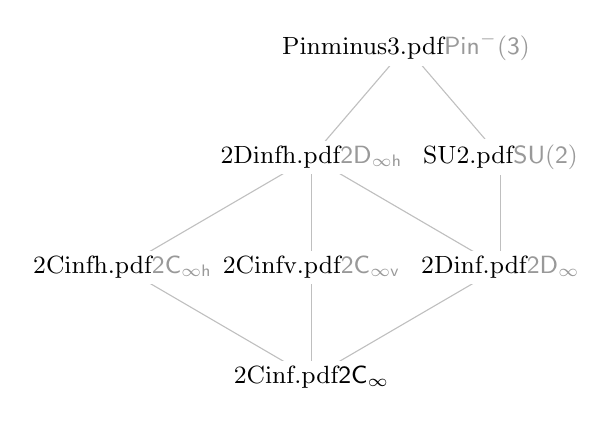
\begin{tikzpicture}[x=1cm, y=1cm, every node/.style={fill=white, font=\small, inner sep=2pt}]
\draw[black!25, line width=0.4pt] (0,0) -- (-2.4,1.4);
\draw[black!25, line width=0.4pt] (0,0) -- (0,1.4);
\draw[black!25, line width=0.4pt] (0,0) -- (2.4,1.4);
\draw[black!25, line width=0.4pt] (-2.4,1.4) -- (0,2.8);
\draw[black!25, line width=0.4pt] (0,1.4) -- (0,2.8);
\draw[black!25, line width=0.4pt] (2.4,1.4) -- (0,2.8);
\draw[black!25, line width=0.4pt] (2.4,1.4) -- (2.4,2.8);
\draw[black!25, line width=0.4pt] (0,2.8) -- (1.2,4.2);
\draw[black!25, line width=0.4pt] (2.4,2.8) -- (1.2,4.2);
\node at (0,0) {\href{2Cinf.pdf}{\textcolor{black}{$\grp{2C_{\infty }}$}}};
\node at (-2.4,1.4) {\href{2Cinfh.pdf}{\textcolor{black!40}{$\grp{2C_{\infty h}}$}}};
\node at (0,1.4) {\href{2Cinfv.pdf}{\textcolor{black!40}{$\grp{2C_{\infty v}}$}}};
\node at (2.4,1.4) {\href{2Dinf.pdf}{\textcolor{black!40}{$\grp{2D_{\infty }}$}}};
\node at (0,2.8) {\href{2Dinfh.pdf}{\textcolor{black!40}{$\grp{2D_{\infty h}}$}}};
\node at (2.4,2.8) {\href{SU2.pdf}{\textcolor{black!40}{$\grp{SU(2)}$}}};
\node at (1.2,4.2) {\href{Pinminus3.pdf}{\textcolor{black!40}{$\grp{Pin^{-}(3)}$}}};
\end{tikzpicture}\end{center}
The table lists the preimages and the sections of each family. \label{n:index.family.N}A row with $N$ in its symbol stands for every $N$ of its range, and its entries are functions of $N$. \label{n:head.subgroup}\label{n:head.order}\label{n:head.conjugates}\label{n:head.normal}A row gives the representative of a class of subgroups (subgrp), its order, the number of subgroups conjugate to it (conjugates) and whether it is normal. \label{n:head.normalizer}\label{n:head.centralizer}It also gives its normalizer and its centralizer in $\grp{2C_{\infty }}$. The record holds the members with $N \le 12$ (\texttt{subduction\symbol{95}subgroups}).
{\small\begin{longtable}{@{}lrrlll@{}}\toprule
subgrp & order & conjugates & normal & normalizer & centralizer\\\midrule\endhead
\bottomrule\endfoot\endlastfoot
$\grp{2C_{\mathnormal{N}}}$, $N \ge 1$ & $2N$ & 1 & yes & \href{2Cinf.pdf}{$\grp{2C_{\infty }}$} & \href{2Cinf.pdf}{$\grp{2C_{\infty }}$}\\*
$\grp{C_{\mathnormal{N}}}$, $N \ge 1$ odd & $N$ & 1 & yes & \href{2Cinf.pdf}{$\grp{2C_{\infty }}$} & \href{2Cinf.pdf}{$\grp{2C_{\infty }}$}\\
\bottomrule\end{longtable}}
\needspace{169pt}
\section{Descent of symmetry}\label{s:subduction}
Conventions: \href{../../CONVENTIONS.pdf}{CONVENTIONS.pdf}, sections \href{../../../rotation/CONVENTIONS.pdf\#conv.16.1}{16.1} and \href{../../CONVENTIONS.pdf\#conv.29.5}{29.5}.
\needspace{116pt}
\paragraph{Vector families.} The vector families of $\grp{2C_{\infty }}$ are those of \href{../../../rotation/data/pdf/Cinf.pdf}{$\grp{C_{\infty}}$}. They restrict to the preimage $\grp{2H}$ of a closed subgroup $\grp{H}$ of \href{../../../rotation/data/pdf/Cinf.pdf}{$\grp{C_{\infty}}$} as \href{../../../rotation/data/pdf/Cinf.pdf}{$\grp{C_{\infty}}$} restricts them to $\grp{H}$ (\texttt{vector\symbol{95}entry}, \texttt{vector\symbol{95}rules}), whose irreps are the vector irreps of $\grp{2H}$. The families restrict to a section as to its preimage. The tables are those of the section Descent of symmetry of the document of \href{../../../rotation/data/pdf/Cinf.pdf}{$\grp{C_{\infty}}$}, with its settings. They are headed by the preimages and give the images of the generators of $\grp{H}$ at the points of the class space (section~\ref{s:class_space}). \label{n:irrep.Gamma.subgroup}The entry of row $\Gamma$ is $\restr{\Gamma}{\grp{H}}$ as a sum of the irreps of $\grp{H}$.

\needspace{95pt}
\paragraph{Vector families, the $\grp{2C_{\mathnormal{N}}}$ family.}
{\small\setlength{\fillwidth}{\textwidth}\addtolength{\fillwidth}{-2\tabcolsep}\setlength{\colwidth}{0pt}\cellmax{$\conjpair{1}\irr{e}_{n}$}\cellmax{$\conjpair{2}\irr{e}_{n}$}\cellmax{$\irr{a}$}\addtolength{\fillwidth}{-\colwidth}\setlength{\colwidth}{0pt}\cellmax{$\irr{a}$ if $q = 0$, $\irr{b}$ if $q = N/2$, $\conjpair{1}\irr{e}_{q}$ if $0 < q < N/2$, $\conjpair{2}\irr{e}_{N-q}$ if $N/2 < q < N$; $q = -n \bmod N$}\cellmax{$\irr{a}$ if $q = 0$, $\irr{b}$ if $q = N/2$, $\conjpair{1}\irr{e}_{q}$ if $0 < q < N/2$, $\conjpair{2}\irr{e}_{N-q}$ if $N/2 < q < N$; $q = n \bmod N$}\cellmax{$\irr{a}$}\fillcap\begin{longtable}{@{}l>{\raggedright\arraybackslash}p{\fillwidth}@{}}\toprule
\multicolumn{2}{@{}c@{}}{every $N$}\\*
$\irr{a}$ & $\irr{a}$\\*
$\conjpair{1}\irr{e}_{n}$ & $\irr{a}$ if $q = 0$, $\irr{b}$ if $q = N/2$, $\conjpair{1}\irr{e}_{q}$ if $0 < q < N/2$, $\conjpair{2}\irr{e}_{N-q}$ if $N/2 < q < N$; $q = n \bmod N$\\*
$\conjpair{2}\irr{e}_{n}$ & $\irr{a}$ if $q = 0$, $\irr{b}$ if $q = N/2$, $\conjpair{1}\irr{e}_{q}$ if $0 < q < N/2$, $\conjpair{2}\irr{e}_{N-q}$ if $N/2 < q < N$; $q = -n \bmod N$\\
\bottomrule\end{longtable}}
{\small\begin{longtable}{@{}lccccccc@{}}\toprule
subgrp & \href{2C2.pdf}{$\grp{2C_{2}}$} & \multicolumn{2}{c}{\href{2C3.pdf}{$\grp{2C_{3}}$}} & \multicolumn{2}{c}{\href{2C4.pdf}{$\grp{2C_{4}}$}} & \multicolumn{2}{c}{\href{2C5.pdf}{$\grp{2C_{5}}$}}\\\cmidrule(lr){3-4}\cmidrule(lr){5-6}\cmidrule(lr){7-8}
setting &  & 1 & 2 & 1 & 2 & 1 & 2\\
images &  & {\scriptsize $\cls{C_{3}} \mapsto \elt{\lift{C}}(2\pi/3)$} & {\scriptsize $\cls{C_{3}} \mapsto \elt{\lift{C}}(4\pi/3)$} & {\scriptsize $\cls{C_{4}} \mapsto \elt{\lift{C}}(\pi/2)$} & {\scriptsize $\cls{C_{4}} \mapsto \elt{\lift{C}}(3\pi/2)$} & {\scriptsize $\cls{C_{5}} \mapsto \elt{\lift{C}}(2\pi/5)$} & {\scriptsize $\cls{C_{5}} \mapsto \elt{\lift{C}}(8\pi/5)$}\\\midrule\endhead
\bottomrule\endfoot\endlastfoot
$\irr{a}$ & $\irr{a}$ & $\irr{a}$ & $\irr{a}$ & $\irr{a}$ & $\irr{a}$ & $\irr{a}$ & $\irr{a}$\\*
$\conjpair{1}\irr{e}_{1}$ & $\irr{b}$ & $\conjpair{1}\irr{e}$ & $\conjpair{2}\irr{e}$ & $\conjpair{1}\irr{e}$ & $\conjpair{2}\irr{e}$ & $\conjpair{1}\irr{e}_{1}$ & $\conjpair{2}\irr{e}_{1}$\\
$\conjpair{1}\irr{e}_{2}$ & $\irr{a}$ & $\conjpair{2}\irr{e}$ & $\conjpair{1}\irr{e}$ & $\irr{b}$ & $\irr{b}$ & $\conjpair{1}\irr{e}_{2}$ & $\conjpair{2}\irr{e}_{2}$\\
$\conjpair{1}\irr{e}_{3}$ & $\irr{b}$ & $\irr{a}$ & $\irr{a}$ & $\conjpair{2}\irr{e}$ & $\conjpair{1}\irr{e}$ & $\conjpair{2}\irr{e}_{2}$ & $\conjpair{1}\irr{e}_{2}$\\
$\conjpair{1}\irr{e}_{4}$ & $\irr{a}$ & $\conjpair{1}\irr{e}$ & $\conjpair{2}\irr{e}$ & $\irr{a}$ & $\irr{a}$ & $\conjpair{2}\irr{e}_{1}$ & $\conjpair{1}\irr{e}_{1}$\\
$\conjpair{1}\irr{e}_{5}$ & $\irr{b}$ & $\conjpair{2}\irr{e}$ & $\conjpair{1}\irr{e}$ & $\conjpair{1}\irr{e}$ & $\conjpair{2}\irr{e}$ & $\irr{a}$ & $\irr{a}$\\
$\conjpair{1}\irr{e}_{6}$ & $\irr{a}$ & $\irr{a}$ & $\irr{a}$ & $\irr{b}$ & $\irr{b}$ & $\conjpair{1}\irr{e}_{1}$ & $\conjpair{2}\irr{e}_{1}$\\
$\conjpair{2}\irr{e}_{1}$ & $\irr{b}$ & $\conjpair{2}\irr{e}$ & $\conjpair{1}\irr{e}$ & $\conjpair{2}\irr{e}$ & $\conjpair{1}\irr{e}$ & $\conjpair{2}\irr{e}_{1}$ & $\conjpair{1}\irr{e}_{1}$\\
$\conjpair{2}\irr{e}_{2}$ & $\irr{a}$ & $\conjpair{1}\irr{e}$ & $\conjpair{2}\irr{e}$ & $\irr{b}$ & $\irr{b}$ & $\conjpair{2}\irr{e}_{2}$ & $\conjpair{1}\irr{e}_{2}$\\
$\conjpair{2}\irr{e}_{3}$ & $\irr{b}$ & $\irr{a}$ & $\irr{a}$ & $\conjpair{1}\irr{e}$ & $\conjpair{2}\irr{e}$ & $\conjpair{1}\irr{e}_{2}$ & $\conjpair{2}\irr{e}_{2}$\\
$\conjpair{2}\irr{e}_{4}$ & $\irr{a}$ & $\conjpair{2}\irr{e}$ & $\conjpair{1}\irr{e}$ & $\irr{a}$ & $\irr{a}$ & $\conjpair{1}\irr{e}_{1}$ & $\conjpair{2}\irr{e}_{1}$\\
$\conjpair{2}\irr{e}_{5}$ & $\irr{b}$ & $\conjpair{1}\irr{e}$ & $\conjpair{2}\irr{e}$ & $\conjpair{2}\irr{e}$ & $\conjpair{1}\irr{e}$ & $\irr{a}$ & $\irr{a}$\\*
$\conjpair{2}\irr{e}_{6}$ & $\irr{a}$ & $\irr{a}$ & $\irr{a}$ & $\irr{b}$ & $\irr{b}$ & $\conjpair{2}\irr{e}_{1}$ & $\conjpair{1}\irr{e}_{1}$\\
\bottomrule\end{longtable}}
{\small\begin{longtable}{@{}lcccccc@{}}\toprule
subgrp & \multicolumn{2}{c}{\href{2C6.pdf}{$\grp{2C_{6}}$}} & \multicolumn{2}{c}{\href{2C7.pdf}{$\grp{2C_{7}}$}} & \multicolumn{2}{c}{\href{2C8.pdf}{$\grp{2C_{8}}$}}\\\cmidrule(lr){2-3}\cmidrule(lr){4-5}\cmidrule(lr){6-7}
setting & 1 & 2 & 1 & 2 & 1 & 2\\
images & {\scriptsize $\cls{C_{6}} \mapsto \elt{\lift{C}}(\pi/3)$} & {\scriptsize $\cls{C_{6}} \mapsto \elt{\lift{C}}(5\pi/3)$} & {\scriptsize $\cls{C_{7}} \mapsto \elt{\lift{C}}(2\pi/7)$} & {\scriptsize $\cls{C_{7}} \mapsto \elt{\lift{C}}(12\pi/7)$} & {\scriptsize $\cls{C_{8}} \mapsto \elt{\lift{C}}(\pi/4)$} & {\scriptsize $\cls{C_{8}} \mapsto \elt{\lift{C}}(7\pi/4)$}\\\midrule\endhead
\bottomrule\endfoot\endlastfoot
$\irr{a}$ & $\irr{a}$ & $\irr{a}$ & $\irr{a}$ & $\irr{a}$ & $\irr{a}$ & $\irr{a}$\\*
$\conjpair{1}\irr{e}_{1}$ & $\conjpair{1}\irr{e}_{1}$ & $\conjpair{2}\irr{e}_{1}$ & $\conjpair{1}\irr{e}_{1}$ & $\conjpair{2}\irr{e}_{1}$ & $\conjpair{1}\irr{e}_{1}$ & $\conjpair{2}\irr{e}_{1}$\\
$\conjpair{1}\irr{e}_{2}$ & $\conjpair{1}\irr{e}_{2}$ & $\conjpair{2}\irr{e}_{2}$ & $\conjpair{1}\irr{e}_{2}$ & $\conjpair{2}\irr{e}_{2}$ & $\conjpair{1}\irr{e}_{2}$ & $\conjpair{2}\irr{e}_{2}$\\
$\conjpair{1}\irr{e}_{3}$ & $\irr{b}$ & $\irr{b}$ & $\conjpair{1}\irr{e}_{3}$ & $\conjpair{2}\irr{e}_{3}$ & $\conjpair{1}\irr{e}_{3}$ & $\conjpair{2}\irr{e}_{3}$\\
$\conjpair{1}\irr{e}_{4}$ & $\conjpair{2}\irr{e}_{2}$ & $\conjpair{1}\irr{e}_{2}$ & $\conjpair{2}\irr{e}_{3}$ & $\conjpair{1}\irr{e}_{3}$ & $\irr{b}$ & $\irr{b}$\\
$\conjpair{1}\irr{e}_{5}$ & $\conjpair{2}\irr{e}_{1}$ & $\conjpair{1}\irr{e}_{1}$ & $\conjpair{2}\irr{e}_{2}$ & $\conjpair{1}\irr{e}_{2}$ & $\conjpair{2}\irr{e}_{3}$ & $\conjpair{1}\irr{e}_{3}$\\
$\conjpair{1}\irr{e}_{6}$ & $\irr{a}$ & $\irr{a}$ & $\conjpair{2}\irr{e}_{1}$ & $\conjpair{1}\irr{e}_{1}$ & $\conjpair{2}\irr{e}_{2}$ & $\conjpair{1}\irr{e}_{2}$\\
$\conjpair{2}\irr{e}_{1}$ & $\conjpair{2}\irr{e}_{1}$ & $\conjpair{1}\irr{e}_{1}$ & $\conjpair{2}\irr{e}_{1}$ & $\conjpair{1}\irr{e}_{1}$ & $\conjpair{2}\irr{e}_{1}$ & $\conjpair{1}\irr{e}_{1}$\\
$\conjpair{2}\irr{e}_{2}$ & $\conjpair{2}\irr{e}_{2}$ & $\conjpair{1}\irr{e}_{2}$ & $\conjpair{2}\irr{e}_{2}$ & $\conjpair{1}\irr{e}_{2}$ & $\conjpair{2}\irr{e}_{2}$ & $\conjpair{1}\irr{e}_{2}$\\
$\conjpair{2}\irr{e}_{3}$ & $\irr{b}$ & $\irr{b}$ & $\conjpair{2}\irr{e}_{3}$ & $\conjpair{1}\irr{e}_{3}$ & $\conjpair{2}\irr{e}_{3}$ & $\conjpair{1}\irr{e}_{3}$\\
$\conjpair{2}\irr{e}_{4}$ & $\conjpair{1}\irr{e}_{2}$ & $\conjpair{2}\irr{e}_{2}$ & $\conjpair{1}\irr{e}_{3}$ & $\conjpair{2}\irr{e}_{3}$ & $\irr{b}$ & $\irr{b}$\\
$\conjpair{2}\irr{e}_{5}$ & $\conjpair{1}\irr{e}_{1}$ & $\conjpair{2}\irr{e}_{1}$ & $\conjpair{1}\irr{e}_{2}$ & $\conjpair{2}\irr{e}_{2}$ & $\conjpair{1}\irr{e}_{3}$ & $\conjpair{2}\irr{e}_{3}$\\*
$\conjpair{2}\irr{e}_{6}$ & $\irr{a}$ & $\irr{a}$ & $\conjpair{1}\irr{e}_{1}$ & $\conjpair{2}\irr{e}_{1}$ & $\conjpair{1}\irr{e}_{2}$ & $\conjpair{2}\irr{e}_{2}$\\
\bottomrule\end{longtable}}
{\small\begin{longtable}{@{}lcccc@{}}\toprule
subgrp & \multicolumn{2}{c}{\href{2C9.pdf}{$\grp{2C_{9}}$}} & \multicolumn{2}{c}{\href{2C10.pdf}{$\grp{2C_{10}}$}}\\\cmidrule(lr){2-3}\cmidrule(lr){4-5}
setting & 1 & 2 & 1 & 2\\
images & {\scriptsize $\cls{C_{9}} \mapsto \elt{\lift{C}}(2\pi/9)$} & {\scriptsize $\cls{C_{9}} \mapsto \elt{\lift{C}}(16\pi/9)$} & {\scriptsize $\cls{C_{10}} \mapsto \elt{\lift{C}}(\pi/5)$} & {\scriptsize $\cls{C_{10}} \mapsto \elt{\lift{C}}(9\pi/5)$}\\\midrule\endhead
\bottomrule\endfoot\endlastfoot
$\irr{a}$ & $\irr{a}$ & $\irr{a}$ & $\irr{a}$ & $\irr{a}$\\*
$\conjpair{1}\irr{e}_{1}$ & $\conjpair{1}\irr{e}_{1}$ & $\conjpair{2}\irr{e}_{1}$ & $\conjpair{1}\irr{e}_{1}$ & $\conjpair{2}\irr{e}_{1}$\\
$\conjpair{1}\irr{e}_{2}$ & $\conjpair{1}\irr{e}_{2}$ & $\conjpair{2}\irr{e}_{2}$ & $\conjpair{1}\irr{e}_{2}$ & $\conjpair{2}\irr{e}_{2}$\\
$\conjpair{1}\irr{e}_{3}$ & $\conjpair{1}\irr{e}_{3}$ & $\conjpair{2}\irr{e}_{3}$ & $\conjpair{1}\irr{e}_{3}$ & $\conjpair{2}\irr{e}_{3}$\\
$\conjpair{1}\irr{e}_{4}$ & $\conjpair{1}\irr{e}_{4}$ & $\conjpair{2}\irr{e}_{4}$ & $\conjpair{1}\irr{e}_{4}$ & $\conjpair{2}\irr{e}_{4}$\\
$\conjpair{1}\irr{e}_{5}$ & $\conjpair{2}\irr{e}_{4}$ & $\conjpair{1}\irr{e}_{4}$ & $\irr{b}$ & $\irr{b}$\\
$\conjpair{1}\irr{e}_{6}$ & $\conjpair{2}\irr{e}_{3}$ & $\conjpair{1}\irr{e}_{3}$ & $\conjpair{2}\irr{e}_{4}$ & $\conjpair{1}\irr{e}_{4}$\\
$\conjpair{2}\irr{e}_{1}$ & $\conjpair{2}\irr{e}_{1}$ & $\conjpair{1}\irr{e}_{1}$ & $\conjpair{2}\irr{e}_{1}$ & $\conjpair{1}\irr{e}_{1}$\\
$\conjpair{2}\irr{e}_{2}$ & $\conjpair{2}\irr{e}_{2}$ & $\conjpair{1}\irr{e}_{2}$ & $\conjpair{2}\irr{e}_{2}$ & $\conjpair{1}\irr{e}_{2}$\\
$\conjpair{2}\irr{e}_{3}$ & $\conjpair{2}\irr{e}_{3}$ & $\conjpair{1}\irr{e}_{3}$ & $\conjpair{2}\irr{e}_{3}$ & $\conjpair{1}\irr{e}_{3}$\\
$\conjpair{2}\irr{e}_{4}$ & $\conjpair{2}\irr{e}_{4}$ & $\conjpair{1}\irr{e}_{4}$ & $\conjpair{2}\irr{e}_{4}$ & $\conjpair{1}\irr{e}_{4}$\\
$\conjpair{2}\irr{e}_{5}$ & $\conjpair{1}\irr{e}_{4}$ & $\conjpair{2}\irr{e}_{4}$ & $\irr{b}$ & $\irr{b}$\\*
$\conjpair{2}\irr{e}_{6}$ & $\conjpair{1}\irr{e}_{3}$ & $\conjpair{2}\irr{e}_{3}$ & $\conjpair{1}\irr{e}_{4}$ & $\conjpair{2}\irr{e}_{4}$\\
\bottomrule\end{longtable}}
{\small\begin{longtable}{@{}lcccc@{}}\toprule
subgrp & \multicolumn{2}{c}{\href{2C11.pdf}{$\grp{2C_{11}}$}} & \multicolumn{2}{c}{\href{2C12.pdf}{$\grp{2C_{12}}$}}\\\cmidrule(lr){2-3}\cmidrule(lr){4-5}
setting & 1 & 2 & 1 & 2\\
images & {\scriptsize $\cls{C_{11}} \mapsto \elt{\lift{C}}(2\pi/11)$} & {\scriptsize $\cls{C_{11}} \mapsto \elt{\lift{C}}(20\pi/11)$} & {\scriptsize $\cls{C_{12}} \mapsto \elt{\lift{C}}(\pi/6)$} & {\scriptsize $\cls{C_{12}} \mapsto \elt{\lift{C}}(11\pi/6)$}\\\midrule\endhead
\bottomrule\endfoot\endlastfoot
$\irr{a}$ & $\irr{a}$ & $\irr{a}$ & $\irr{a}$ & $\irr{a}$\\*
$\conjpair{1}\irr{e}_{1}$ & $\conjpair{1}\irr{e}_{1}$ & $\conjpair{2}\irr{e}_{1}$ & $\conjpair{1}\irr{e}_{1}$ & $\conjpair{2}\irr{e}_{1}$\\
$\conjpair{1}\irr{e}_{2}$ & $\conjpair{1}\irr{e}_{2}$ & $\conjpair{2}\irr{e}_{2}$ & $\conjpair{1}\irr{e}_{2}$ & $\conjpair{2}\irr{e}_{2}$\\
$\conjpair{1}\irr{e}_{3}$ & $\conjpair{1}\irr{e}_{3}$ & $\conjpair{2}\irr{e}_{3}$ & $\conjpair{1}\irr{e}_{3}$ & $\conjpair{2}\irr{e}_{3}$\\
$\conjpair{1}\irr{e}_{4}$ & $\conjpair{1}\irr{e}_{4}$ & $\conjpair{2}\irr{e}_{4}$ & $\conjpair{1}\irr{e}_{4}$ & $\conjpair{2}\irr{e}_{4}$\\
$\conjpair{1}\irr{e}_{5}$ & $\conjpair{1}\irr{e}_{5}$ & $\conjpair{2}\irr{e}_{5}$ & $\conjpair{1}\irr{e}_{5}$ & $\conjpair{2}\irr{e}_{5}$\\
$\conjpair{1}\irr{e}_{6}$ & $\conjpair{2}\irr{e}_{5}$ & $\conjpair{1}\irr{e}_{5}$ & $\irr{b}$ & $\irr{b}$\\
$\conjpair{2}\irr{e}_{1}$ & $\conjpair{2}\irr{e}_{1}$ & $\conjpair{1}\irr{e}_{1}$ & $\conjpair{2}\irr{e}_{1}$ & $\conjpair{1}\irr{e}_{1}$\\
$\conjpair{2}\irr{e}_{2}$ & $\conjpair{2}\irr{e}_{2}$ & $\conjpair{1}\irr{e}_{2}$ & $\conjpair{2}\irr{e}_{2}$ & $\conjpair{1}\irr{e}_{2}$\\
$\conjpair{2}\irr{e}_{3}$ & $\conjpair{2}\irr{e}_{3}$ & $\conjpair{1}\irr{e}_{3}$ & $\conjpair{2}\irr{e}_{3}$ & $\conjpair{1}\irr{e}_{3}$\\
$\conjpair{2}\irr{e}_{4}$ & $\conjpair{2}\irr{e}_{4}$ & $\conjpair{1}\irr{e}_{4}$ & $\conjpair{2}\irr{e}_{4}$ & $\conjpair{1}\irr{e}_{4}$\\
$\conjpair{2}\irr{e}_{5}$ & $\conjpair{2}\irr{e}_{5}$ & $\conjpair{1}\irr{e}_{5}$ & $\conjpair{2}\irr{e}_{5}$ & $\conjpair{1}\irr{e}_{5}$\\*
$\conjpair{2}\irr{e}_{6}$ & $\conjpair{1}\irr{e}_{5}$ & $\conjpair{2}\irr{e}_{5}$ & $\irr{b}$ & $\irr{b}$\\
\bottomrule\end{longtable}}

\needspace{101pt}
\paragraph{Spinor families.} Below is the restriction of the spinor families to the finite subgroups that the rules and the tables list.
\leavevmode\label{n:index.residue}For the preimage $\grp{2C_{\mathnormal{N}}}$, the rules give it for every $N$ by $q$ ($0 < q < N$):
{\small\begin{longtable}{@{}ll>{\RaggedRight\arraybackslash}p{0.7\textwidth}@{}}\toprule
subgrp & family & irreps\\\midrule\endhead
\bottomrule\endfoot\endlastfoot
$\grp{2C_{\mathnormal{N}}}$ & $\conjpair{1}\irr{e}_{n}$ & $\conjpair{1}\irr{e}_{q}$ if $q < N/2$, $\irr{a}_{N/2}$ if $q = N/2$, $\conjpair{2}\irr{e}_{N-q}$ if $q > N/2$; $q = n \bmod N$\\*
$\grp{2C_{\mathnormal{N}}}$ & $\conjpair{2}\irr{e}_{n}$ & $\conjpair{1}\irr{e}_{q}$ if $q < N/2$, $\irr{a}_{N/2}$ if $q = N/2$, $\conjpair{2}\irr{e}_{N-q}$ if $q > N/2$; $q = -n \bmod N$\\
\bottomrule\end{longtable}}
For a finite subgroup the restriction of the instance $n$ depends on $n$ only modulo its period $P$. The table lists the finite preimages with $N \le 12$ and gives, for $n = \tfrac{1}{2}, \tfrac{3}{2}, \dots, P - \tfrac{1}{2}$, the irreps of the subgroup, and the record holds the intertwiners (\texttt{blocks}). A section is restricted as its preimage, with each spinor irrep renamed by the section's record (\href{../../CONVENTIONS.pdf}{CONVENTIONS.pdf}, section \href{../../CONVENTIONS.pdf\#conv.27}{27}).
{\small\setlength{\fillwidth}{\textwidth}\addtolength{\fillwidth}{-6\tabcolsep}\setlength{\colwidth}{0pt}\cellmax{subgrp}\cellmax{$\grp{2C_{10}}$}\cellmax{$\grp{2C_{11}}$}\cellmax{$\grp{2C_{12}}$}\cellmax{$\grp{2C_{1}}$}\cellmax{$\grp{2C_{2}}$}\cellmax{$\grp{2C_{3}}$}\cellmax{$\grp{2C_{4}}$}\cellmax{$\grp{2C_{5}}$}\cellmax{$\grp{2C_{6}}$}\cellmax{$\grp{2C_{7}}$}\cellmax{$\grp{2C_{8}}$}\cellmax{$\grp{2C_{9}}$}\addtolength{\fillwidth}{-\colwidth}\setlength{\colwidth}{0pt}\cellmax{family}\cellmax{$\conjpair{1}\irr{e}_{n}$}\cellmax{$\conjpair{2}\irr{e}_{n}$}\addtolength{\fillwidth}{-\colwidth}\setlength{\colwidth}{0pt}\cellmax{10}\cellmax{11}\cellmax{12}\cellmax{$P$}\cellmax{1}\cellmax{2}\cellmax{3}\cellmax{4}\cellmax{5}\cellmax{6}\cellmax{7}\cellmax{8}\cellmax{9}\addtolength{\fillwidth}{-\colwidth}\setlength{\colwidth}{0pt}\cellmax{$\nicefrac{1}{2}$: $\conjpair{1}\irr{e}_{1/2}$; $\nicefrac{3}{2}$: $\conjpair{1}\irr{e}_{3/2}$; $\nicefrac{5}{2}$: $\conjpair{1}\irr{e}_{5/2}$; $\nicefrac{7}{2}$: $\conjpair{1}\irr{e}_{7/2}$; $\nicefrac{9}{2}$: $\conjpair{1}\irr{e}_{9/2}$; $\nicefrac{11}{2}$: $\conjpair{1}\irr{e}_{11/2}$; $\nicefrac{13}{2}$: $\conjpair{2}\irr{e}_{11/2}$; $\nicefrac{15}{2}$: $\conjpair{2}\irr{e}_{9/2}$; $\nicefrac{17}{2}$: $\conjpair{2}\irr{e}_{7/2}$; $\nicefrac{19}{2}$: $\conjpair{2}\irr{e}_{5/2}$; $\nicefrac{21}{2}$: $\conjpair{2}\irr{e}_{3/2}$; $\nicefrac{23}{2}$: $\conjpair{2}\irr{e}_{1/2}$}\cellmax{$\nicefrac{1}{2}$: $\conjpair{2}\irr{e}_{1/2}$; $\nicefrac{3}{2}$: $\conjpair{2}\irr{e}_{3/2}$; $\nicefrac{5}{2}$: $\conjpair{2}\irr{e}_{5/2}$; $\nicefrac{7}{2}$: $\conjpair{2}\irr{e}_{7/2}$; $\nicefrac{9}{2}$: $\conjpair{2}\irr{e}_{9/2}$; $\nicefrac{11}{2}$: $\conjpair{2}\irr{e}_{11/2}$; $\nicefrac{13}{2}$: $\conjpair{1}\irr{e}_{11/2}$; $\nicefrac{15}{2}$: $\conjpair{1}\irr{e}_{9/2}$; $\nicefrac{17}{2}$: $\conjpair{1}\irr{e}_{7/2}$; $\nicefrac{19}{2}$: $\conjpair{1}\irr{e}_{5/2}$; $\nicefrac{21}{2}$: $\conjpair{1}\irr{e}_{3/2}$; $\nicefrac{23}{2}$: $\conjpair{1}\irr{e}_{1/2}$}\cellmax{$\nicefrac{1}{2}$: $\conjpair{1}\irr{e}_{1/2}$; $\nicefrac{3}{2}$: $\conjpair{1}\irr{e}_{3/2}$; $\nicefrac{5}{2}$: $\conjpair{1}\irr{e}_{5/2}$; $\nicefrac{7}{2}$: $\conjpair{1}\irr{e}_{7/2}$; $\nicefrac{9}{2}$: $\conjpair{1}\irr{e}_{9/2}$; $\nicefrac{11}{2}$: $\irr{a}_{11/2}$; $\nicefrac{13}{2}$: $\conjpair{2}\irr{e}_{9/2}$; $\nicefrac{15}{2}$: $\conjpair{2}\irr{e}_{7/2}$; $\nicefrac{17}{2}$: $\conjpair{2}\irr{e}_{5/2}$; $\nicefrac{19}{2}$: $\conjpair{2}\irr{e}_{3/2}$; $\nicefrac{21}{2}$: $\conjpair{2}\irr{e}_{1/2}$}\cellmax{$\nicefrac{1}{2}$: $\conjpair{2}\irr{e}_{1/2}$; $\nicefrac{3}{2}$: $\conjpair{2}\irr{e}_{3/2}$; $\nicefrac{5}{2}$: $\conjpair{2}\irr{e}_{5/2}$; $\nicefrac{7}{2}$: $\conjpair{2}\irr{e}_{7/2}$; $\nicefrac{9}{2}$: $\conjpair{2}\irr{e}_{9/2}$; $\nicefrac{11}{2}$: $\irr{a}_{11/2}$; $\nicefrac{13}{2}$: $\conjpair{1}\irr{e}_{9/2}$; $\nicefrac{15}{2}$: $\conjpair{1}\irr{e}_{7/2}$; $\nicefrac{17}{2}$: $\conjpair{1}\irr{e}_{5/2}$; $\nicefrac{19}{2}$: $\conjpair{1}\irr{e}_{3/2}$; $\nicefrac{21}{2}$: $\conjpair{1}\irr{e}_{1/2}$}\cellmax{$\nicefrac{1}{2}$: $\conjpair{1}\irr{e}_{1/2}$; $\nicefrac{3}{2}$: $\conjpair{1}\irr{e}_{3/2}$; $\nicefrac{5}{2}$: $\conjpair{1}\irr{e}_{5/2}$; $\nicefrac{7}{2}$: $\conjpair{1}\irr{e}_{7/2}$; $\nicefrac{9}{2}$: $\conjpair{1}\irr{e}_{9/2}$; $\nicefrac{11}{2}$: $\conjpair{2}\irr{e}_{9/2}$; $\nicefrac{13}{2}$: $\conjpair{2}\irr{e}_{7/2}$; $\nicefrac{15}{2}$: $\conjpair{2}\irr{e}_{5/2}$; $\nicefrac{17}{2}$: $\conjpair{2}\irr{e}_{3/2}$; $\nicefrac{19}{2}$: $\conjpair{2}\irr{e}_{1/2}$}\cellmax{$\nicefrac{1}{2}$: $\conjpair{2}\irr{e}_{1/2}$; $\nicefrac{3}{2}$: $\conjpair{2}\irr{e}_{3/2}$; $\nicefrac{5}{2}$: $\conjpair{2}\irr{e}_{5/2}$; $\nicefrac{7}{2}$: $\conjpair{2}\irr{e}_{7/2}$; $\nicefrac{9}{2}$: $\conjpair{2}\irr{e}_{9/2}$; $\nicefrac{11}{2}$: $\conjpair{1}\irr{e}_{9/2}$; $\nicefrac{13}{2}$: $\conjpair{1}\irr{e}_{7/2}$; $\nicefrac{15}{2}$: $\conjpair{1}\irr{e}_{5/2}$; $\nicefrac{17}{2}$: $\conjpair{1}\irr{e}_{3/2}$; $\nicefrac{19}{2}$: $\conjpair{1}\irr{e}_{1/2}$}\cellmax{$\nicefrac{1}{2}$: $\conjpair{1}\irr{e}_{1/2}$; $\nicefrac{3}{2}$: $\conjpair{1}\irr{e}_{3/2}$; $\nicefrac{5}{2}$: $\conjpair{1}\irr{e}_{5/2}$; $\nicefrac{7}{2}$: $\conjpair{1}\irr{e}_{7/2}$; $\nicefrac{9}{2}$: $\irr{a}_{9/2}$; $\nicefrac{11}{2}$: $\conjpair{2}\irr{e}_{7/2}$; $\nicefrac{13}{2}$: $\conjpair{2}\irr{e}_{5/2}$; $\nicefrac{15}{2}$: $\conjpair{2}\irr{e}_{3/2}$; $\nicefrac{17}{2}$: $\conjpair{2}\irr{e}_{1/2}$}\cellmax{$\nicefrac{1}{2}$: $\conjpair{2}\irr{e}_{1/2}$; $\nicefrac{3}{2}$: $\conjpair{2}\irr{e}_{3/2}$; $\nicefrac{5}{2}$: $\conjpair{2}\irr{e}_{5/2}$; $\nicefrac{7}{2}$: $\conjpair{2}\irr{e}_{7/2}$; $\nicefrac{9}{2}$: $\irr{a}_{9/2}$; $\nicefrac{11}{2}$: $\conjpair{1}\irr{e}_{7/2}$; $\nicefrac{13}{2}$: $\conjpair{1}\irr{e}_{5/2}$; $\nicefrac{15}{2}$: $\conjpair{1}\irr{e}_{3/2}$; $\nicefrac{17}{2}$: $\conjpair{1}\irr{e}_{1/2}$}\cellmax{$\nicefrac{1}{2}$: $\conjpair{1}\irr{e}_{1/2}$; $\nicefrac{3}{2}$: $\conjpair{1}\irr{e}_{3/2}$; $\nicefrac{5}{2}$: $\conjpair{1}\irr{e}_{5/2}$; $\nicefrac{7}{2}$: $\conjpair{1}\irr{e}_{7/2}$; $\nicefrac{9}{2}$: $\conjpair{2}\irr{e}_{7/2}$; $\nicefrac{11}{2}$: $\conjpair{2}\irr{e}_{5/2}$; $\nicefrac{13}{2}$: $\conjpair{2}\irr{e}_{3/2}$; $\nicefrac{15}{2}$: $\conjpair{2}\irr{e}_{1/2}$}\cellmax{$\nicefrac{1}{2}$: $\conjpair{2}\irr{e}_{1/2}$; $\nicefrac{3}{2}$: $\conjpair{2}\irr{e}_{3/2}$; $\nicefrac{5}{2}$: $\conjpair{2}\irr{e}_{5/2}$; $\nicefrac{7}{2}$: $\conjpair{2}\irr{e}_{7/2}$; $\nicefrac{9}{2}$: $\conjpair{1}\irr{e}_{7/2}$; $\nicefrac{11}{2}$: $\conjpair{1}\irr{e}_{5/2}$; $\nicefrac{13}{2}$: $\conjpair{1}\irr{e}_{3/2}$; $\nicefrac{15}{2}$: $\conjpair{1}\irr{e}_{1/2}$}\cellmax{$\nicefrac{1}{2}$: $\conjpair{1}\irr{e}_{1/2}$; $\nicefrac{3}{2}$: $\conjpair{1}\irr{e}_{3/2}$; $\nicefrac{5}{2}$: $\conjpair{1}\irr{e}_{5/2}$; $\nicefrac{7}{2}$: $\irr{a}_{7/2}$; $\nicefrac{9}{2}$: $\conjpair{2}\irr{e}_{5/2}$; $\nicefrac{11}{2}$: $\conjpair{2}\irr{e}_{3/2}$; $\nicefrac{13}{2}$: $\conjpair{2}\irr{e}_{1/2}$}\cellmax{$\nicefrac{1}{2}$: $\conjpair{2}\irr{e}_{1/2}$; $\nicefrac{3}{2}$: $\conjpair{2}\irr{e}_{3/2}$; $\nicefrac{5}{2}$: $\conjpair{2}\irr{e}_{5/2}$; $\nicefrac{7}{2}$: $\irr{a}_{7/2}$; $\nicefrac{9}{2}$: $\conjpair{1}\irr{e}_{5/2}$; $\nicefrac{11}{2}$: $\conjpair{1}\irr{e}_{3/2}$; $\nicefrac{13}{2}$: $\conjpair{1}\irr{e}_{1/2}$}\cellmax{$\nicefrac{1}{2}$: $\conjpair{1}\irr{e}_{1/2}$; $\nicefrac{3}{2}$: $\conjpair{1}\irr{e}_{3/2}$; $\nicefrac{5}{2}$: $\conjpair{1}\irr{e}_{5/2}$; $\nicefrac{7}{2}$: $\conjpair{2}\irr{e}_{5/2}$; $\nicefrac{9}{2}$: $\conjpair{2}\irr{e}_{3/2}$; $\nicefrac{11}{2}$: $\conjpair{2}\irr{e}_{1/2}$}\cellmax{$\nicefrac{1}{2}$: $\conjpair{2}\irr{e}_{1/2}$; $\nicefrac{3}{2}$: $\conjpair{2}\irr{e}_{3/2}$; $\nicefrac{5}{2}$: $\conjpair{2}\irr{e}_{5/2}$; $\nicefrac{7}{2}$: $\conjpair{1}\irr{e}_{5/2}$; $\nicefrac{9}{2}$: $\conjpair{1}\irr{e}_{3/2}$; $\nicefrac{11}{2}$: $\conjpair{1}\irr{e}_{1/2}$}\cellmax{$\nicefrac{1}{2}$: $\conjpair{1}\irr{e}_{1/2}$; $\nicefrac{3}{2}$: $\conjpair{1}\irr{e}_{3/2}$; $\nicefrac{5}{2}$: $\irr{a}_{5/2}$; $\nicefrac{7}{2}$: $\conjpair{2}\irr{e}_{3/2}$; $\nicefrac{9}{2}$: $\conjpair{2}\irr{e}_{1/2}$}\cellmax{$\nicefrac{1}{2}$: $\conjpair{2}\irr{e}_{1/2}$; $\nicefrac{3}{2}$: $\conjpair{2}\irr{e}_{3/2}$; $\nicefrac{5}{2}$: $\irr{a}_{5/2}$; $\nicefrac{7}{2}$: $\conjpair{1}\irr{e}_{3/2}$; $\nicefrac{9}{2}$: $\conjpair{1}\irr{e}_{1/2}$}\cellmax{$\nicefrac{1}{2}$: $\conjpair{1}\irr{e}_{1/2}$; $\nicefrac{3}{2}$: $\conjpair{1}\irr{e}_{3/2}$; $\nicefrac{5}{2}$: $\conjpair{2}\irr{e}_{3/2}$; $\nicefrac{7}{2}$: $\conjpair{2}\irr{e}_{1/2}$}\cellmax{$\nicefrac{1}{2}$: $\conjpair{2}\irr{e}_{1/2}$; $\nicefrac{3}{2}$: $\conjpair{2}\irr{e}_{3/2}$; $\nicefrac{5}{2}$: $\conjpair{1}\irr{e}_{3/2}$; $\nicefrac{7}{2}$: $\conjpair{1}\irr{e}_{1/2}$}\cellmax{$\nicefrac{1}{2}$: $\conjpair{1}\irr{e}_{1/2}$; $\nicefrac{3}{2}$: $\irr{a}_{3/2}$; $\nicefrac{5}{2}$: $\conjpair{2}\irr{e}_{1/2}$}\cellmax{$\nicefrac{1}{2}$: $\conjpair{2}\irr{e}_{1/2}$; $\nicefrac{3}{2}$: $\irr{a}_{3/2}$; $\nicefrac{5}{2}$: $\conjpair{1}\irr{e}_{1/2}$}\cellmax{$\nicefrac{1}{2}$: $\conjpair{1}\irr{e}_{1/2}$; $\nicefrac{3}{2}$: $\conjpair{2}\irr{e}_{1/2}$}\cellmax{$\nicefrac{1}{2}$: $\conjpair{2}\irr{e}_{1/2}$; $\nicefrac{3}{2}$: $\conjpair{1}\irr{e}_{1/2}$}\cellmax{$\nicefrac{1}{2}$: $\irr{a}_{1/2}$}\cellmax{irreps}\fillcap\begin{longtable}{@{}llr>{\RaggedRight\arraybackslash}p{\fillwidth}@{}}\toprule
subgrp & family & $P$ & irreps\\\midrule\endhead
\bottomrule\endfoot\endlastfoot
\href{2C1.pdf}{$\grp{2C_{1}}$} & $\conjpair{1}\irr{e}_{n}$ & 1 & $\nicefrac{1}{2}$: $\irr{a}_{1/2}$\\*
\href{2C1.pdf}{$\grp{2C_{1}}$} & $\conjpair{2}\irr{e}_{n}$ & 1 & $\nicefrac{1}{2}$: $\irr{a}_{1/2}$\\
\href{2C2.pdf}{$\grp{2C_{2}}$} & $\conjpair{1}\irr{e}_{n}$ & 2 & $\nicefrac{1}{2}$: $\conjpair{1}\irr{e}_{1/2}$; $\nicefrac{3}{2}$: $\conjpair{2}\irr{e}_{1/2}$\\
\href{2C2.pdf}{$\grp{2C_{2}}$} & $\conjpair{2}\irr{e}_{n}$ & 2 & $\nicefrac{1}{2}$: $\conjpair{2}\irr{e}_{1/2}$; $\nicefrac{3}{2}$: $\conjpair{1}\irr{e}_{1/2}$\\
\href{2C3.pdf}{$\grp{2C_{3}}$} & $\conjpair{1}\irr{e}_{n}$ & 3 & $\nicefrac{1}{2}$: $\conjpair{1}\irr{e}_{1/2}$; $\nicefrac{3}{2}$: $\irr{a}_{3/2}$; $\nicefrac{5}{2}$: $\conjpair{2}\irr{e}_{1/2}$\\
\href{2C3.pdf}{$\grp{2C_{3}}$} & $\conjpair{2}\irr{e}_{n}$ & 3 & $\nicefrac{1}{2}$: $\conjpair{2}\irr{e}_{1/2}$; $\nicefrac{3}{2}$: $\irr{a}_{3/2}$; $\nicefrac{5}{2}$: $\conjpair{1}\irr{e}_{1/2}$\\
\href{2C4.pdf}{$\grp{2C_{4}}$} & $\conjpair{1}\irr{e}_{n}$ & 4 & $\nicefrac{1}{2}$: $\conjpair{1}\irr{e}_{1/2}$; $\nicefrac{3}{2}$: $\conjpair{1}\irr{e}_{3/2}$; $\nicefrac{5}{2}$: $\conjpair{2}\irr{e}_{3/2}$; $\nicefrac{7}{2}$: $\conjpair{2}\irr{e}_{1/2}$\\
\href{2C4.pdf}{$\grp{2C_{4}}$} & $\conjpair{2}\irr{e}_{n}$ & 4 & $\nicefrac{1}{2}$: $\conjpair{2}\irr{e}_{1/2}$; $\nicefrac{3}{2}$: $\conjpair{2}\irr{e}_{3/2}$; $\nicefrac{5}{2}$: $\conjpair{1}\irr{e}_{3/2}$; $\nicefrac{7}{2}$: $\conjpair{1}\irr{e}_{1/2}$\\
\href{2C5.pdf}{$\grp{2C_{5}}$} & $\conjpair{1}\irr{e}_{n}$ & 5 & $\nicefrac{1}{2}$: $\conjpair{1}\irr{e}_{1/2}$; $\nicefrac{3}{2}$: $\conjpair{1}\irr{e}_{3/2}$; $\nicefrac{5}{2}$: $\irr{a}_{5/2}$; $\nicefrac{7}{2}$: $\conjpair{2}\irr{e}_{3/2}$; $\nicefrac{9}{2}$: $\conjpair{2}\irr{e}_{1/2}$\\
\href{2C5.pdf}{$\grp{2C_{5}}$} & $\conjpair{2}\irr{e}_{n}$ & 5 & $\nicefrac{1}{2}$: $\conjpair{2}\irr{e}_{1/2}$; $\nicefrac{3}{2}$: $\conjpair{2}\irr{e}_{3/2}$; $\nicefrac{5}{2}$: $\irr{a}_{5/2}$; $\nicefrac{7}{2}$: $\conjpair{1}\irr{e}_{3/2}$; $\nicefrac{9}{2}$: $\conjpair{1}\irr{e}_{1/2}$\\
\href{2C6.pdf}{$\grp{2C_{6}}$} & $\conjpair{1}\irr{e}_{n}$ & 6 & $\nicefrac{1}{2}$: $\conjpair{1}\irr{e}_{1/2}$; $\nicefrac{3}{2}$: $\conjpair{1}\irr{e}_{3/2}$; $\nicefrac{5}{2}$: $\conjpair{1}\irr{e}_{5/2}$; $\nicefrac{7}{2}$: $\conjpair{2}\irr{e}_{5/2}$; $\nicefrac{9}{2}$: $\conjpair{2}\irr{e}_{3/2}$; $\nicefrac{11}{2}$: $\conjpair{2}\irr{e}_{1/2}$\\
\href{2C6.pdf}{$\grp{2C_{6}}$} & $\conjpair{2}\irr{e}_{n}$ & 6 & $\nicefrac{1}{2}$: $\conjpair{2}\irr{e}_{1/2}$; $\nicefrac{3}{2}$: $\conjpair{2}\irr{e}_{3/2}$; $\nicefrac{5}{2}$: $\conjpair{2}\irr{e}_{5/2}$; $\nicefrac{7}{2}$: $\conjpair{1}\irr{e}_{5/2}$; $\nicefrac{9}{2}$: $\conjpair{1}\irr{e}_{3/2}$; $\nicefrac{11}{2}$: $\conjpair{1}\irr{e}_{1/2}$\\
\href{2C7.pdf}{$\grp{2C_{7}}$} & $\conjpair{1}\irr{e}_{n}$ & 7 & $\nicefrac{1}{2}$: $\conjpair{1}\irr{e}_{1/2}$; $\nicefrac{3}{2}$: $\conjpair{1}\irr{e}_{3/2}$; $\nicefrac{5}{2}$: $\conjpair{1}\irr{e}_{5/2}$; $\nicefrac{7}{2}$: $\irr{a}_{7/2}$; $\nicefrac{9}{2}$: $\conjpair{2}\irr{e}_{5/2}$; $\nicefrac{11}{2}$: $\conjpair{2}\irr{e}_{3/2}$; $\nicefrac{13}{2}$: $\conjpair{2}\irr{e}_{1/2}$\\
\href{2C7.pdf}{$\grp{2C_{7}}$} & $\conjpair{2}\irr{e}_{n}$ & 7 & $\nicefrac{1}{2}$: $\conjpair{2}\irr{e}_{1/2}$; $\nicefrac{3}{2}$: $\conjpair{2}\irr{e}_{3/2}$; $\nicefrac{5}{2}$: $\conjpair{2}\irr{e}_{5/2}$; $\nicefrac{7}{2}$: $\irr{a}_{7/2}$; $\nicefrac{9}{2}$: $\conjpair{1}\irr{e}_{5/2}$; $\nicefrac{11}{2}$: $\conjpair{1}\irr{e}_{3/2}$; $\nicefrac{13}{2}$: $\conjpair{1}\irr{e}_{1/2}$\\
\href{2C8.pdf}{$\grp{2C_{8}}$} & $\conjpair{1}\irr{e}_{n}$ & 8 & $\nicefrac{1}{2}$: $\conjpair{1}\irr{e}_{1/2}$; $\nicefrac{3}{2}$: $\conjpair{1}\irr{e}_{3/2}$; $\nicefrac{5}{2}$: $\conjpair{1}\irr{e}_{5/2}$; $\nicefrac{7}{2}$: $\conjpair{1}\irr{e}_{7/2}$; $\nicefrac{9}{2}$: $\conjpair{2}\irr{e}_{7/2}$; $\nicefrac{11}{2}$: $\conjpair{2}\irr{e}_{5/2}$; $\nicefrac{13}{2}$: $\conjpair{2}\irr{e}_{3/2}$; $\nicefrac{15}{2}$: $\conjpair{2}\irr{e}_{1/2}$\\
\href{2C8.pdf}{$\grp{2C_{8}}$} & $\conjpair{2}\irr{e}_{n}$ & 8 & $\nicefrac{1}{2}$: $\conjpair{2}\irr{e}_{1/2}$; $\nicefrac{3}{2}$: $\conjpair{2}\irr{e}_{3/2}$; $\nicefrac{5}{2}$: $\conjpair{2}\irr{e}_{5/2}$; $\nicefrac{7}{2}$: $\conjpair{2}\irr{e}_{7/2}$; $\nicefrac{9}{2}$: $\conjpair{1}\irr{e}_{7/2}$; $\nicefrac{11}{2}$: $\conjpair{1}\irr{e}_{5/2}$; $\nicefrac{13}{2}$: $\conjpair{1}\irr{e}_{3/2}$; $\nicefrac{15}{2}$: $\conjpair{1}\irr{e}_{1/2}$\\
\href{2C9.pdf}{$\grp{2C_{9}}$} & $\conjpair{1}\irr{e}_{n}$ & 9 & $\nicefrac{1}{2}$: $\conjpair{1}\irr{e}_{1/2}$; $\nicefrac{3}{2}$: $\conjpair{1}\irr{e}_{3/2}$; $\nicefrac{5}{2}$: $\conjpair{1}\irr{e}_{5/2}$; $\nicefrac{7}{2}$: $\conjpair{1}\irr{e}_{7/2}$; $\nicefrac{9}{2}$: $\irr{a}_{9/2}$; $\nicefrac{11}{2}$: $\conjpair{2}\irr{e}_{7/2}$; $\nicefrac{13}{2}$: $\conjpair{2}\irr{e}_{5/2}$; $\nicefrac{15}{2}$: $\conjpair{2}\irr{e}_{3/2}$; $\nicefrac{17}{2}$: $\conjpair{2}\irr{e}_{1/2}$\\
\href{2C9.pdf}{$\grp{2C_{9}}$} & $\conjpair{2}\irr{e}_{n}$ & 9 & $\nicefrac{1}{2}$: $\conjpair{2}\irr{e}_{1/2}$; $\nicefrac{3}{2}$: $\conjpair{2}\irr{e}_{3/2}$; $\nicefrac{5}{2}$: $\conjpair{2}\irr{e}_{5/2}$; $\nicefrac{7}{2}$: $\conjpair{2}\irr{e}_{7/2}$; $\nicefrac{9}{2}$: $\irr{a}_{9/2}$; $\nicefrac{11}{2}$: $\conjpair{1}\irr{e}_{7/2}$; $\nicefrac{13}{2}$: $\conjpair{1}\irr{e}_{5/2}$; $\nicefrac{15}{2}$: $\conjpair{1}\irr{e}_{3/2}$; $\nicefrac{17}{2}$: $\conjpair{1}\irr{e}_{1/2}$\\
\href{2C10.pdf}{$\grp{2C_{10}}$} & $\conjpair{1}\irr{e}_{n}$ & 10 & $\nicefrac{1}{2}$: $\conjpair{1}\irr{e}_{1/2}$; $\nicefrac{3}{2}$: $\conjpair{1}\irr{e}_{3/2}$; $\nicefrac{5}{2}$: $\conjpair{1}\irr{e}_{5/2}$; $\nicefrac{7}{2}$: $\conjpair{1}\irr{e}_{7/2}$; $\nicefrac{9}{2}$: $\conjpair{1}\irr{e}_{9/2}$; $\nicefrac{11}{2}$: $\conjpair{2}\irr{e}_{9/2}$; $\nicefrac{13}{2}$: $\conjpair{2}\irr{e}_{7/2}$; $\nicefrac{15}{2}$: $\conjpair{2}\irr{e}_{5/2}$; $\nicefrac{17}{2}$: $\conjpair{2}\irr{e}_{3/2}$; $\nicefrac{19}{2}$: $\conjpair{2}\irr{e}_{1/2}$\\
\href{2C10.pdf}{$\grp{2C_{10}}$} & $\conjpair{2}\irr{e}_{n}$ & 10 & $\nicefrac{1}{2}$: $\conjpair{2}\irr{e}_{1/2}$; $\nicefrac{3}{2}$: $\conjpair{2}\irr{e}_{3/2}$; $\nicefrac{5}{2}$: $\conjpair{2}\irr{e}_{5/2}$; $\nicefrac{7}{2}$: $\conjpair{2}\irr{e}_{7/2}$; $\nicefrac{9}{2}$: $\conjpair{2}\irr{e}_{9/2}$; $\nicefrac{11}{2}$: $\conjpair{1}\irr{e}_{9/2}$; $\nicefrac{13}{2}$: $\conjpair{1}\irr{e}_{7/2}$; $\nicefrac{15}{2}$: $\conjpair{1}\irr{e}_{5/2}$; $\nicefrac{17}{2}$: $\conjpair{1}\irr{e}_{3/2}$; $\nicefrac{19}{2}$: $\conjpair{1}\irr{e}_{1/2}$\\
\href{2C11.pdf}{$\grp{2C_{11}}$} & $\conjpair{1}\irr{e}_{n}$ & 11 & $\nicefrac{1}{2}$: $\conjpair{1}\irr{e}_{1/2}$; $\nicefrac{3}{2}$: $\conjpair{1}\irr{e}_{3/2}$; $\nicefrac{5}{2}$: $\conjpair{1}\irr{e}_{5/2}$; $\nicefrac{7}{2}$: $\conjpair{1}\irr{e}_{7/2}$; $\nicefrac{9}{2}$: $\conjpair{1}\irr{e}_{9/2}$; $\nicefrac{11}{2}$: $\irr{a}_{11/2}$; $\nicefrac{13}{2}$: $\conjpair{2}\irr{e}_{9/2}$; $\nicefrac{15}{2}$: $\conjpair{2}\irr{e}_{7/2}$; $\nicefrac{17}{2}$: $\conjpair{2}\irr{e}_{5/2}$; $\nicefrac{19}{2}$: $\conjpair{2}\irr{e}_{3/2}$; $\nicefrac{21}{2}$: $\conjpair{2}\irr{e}_{1/2}$\\
\href{2C11.pdf}{$\grp{2C_{11}}$} & $\conjpair{2}\irr{e}_{n}$ & 11 & $\nicefrac{1}{2}$: $\conjpair{2}\irr{e}_{1/2}$; $\nicefrac{3}{2}$: $\conjpair{2}\irr{e}_{3/2}$; $\nicefrac{5}{2}$: $\conjpair{2}\irr{e}_{5/2}$; $\nicefrac{7}{2}$: $\conjpair{2}\irr{e}_{7/2}$; $\nicefrac{9}{2}$: $\conjpair{2}\irr{e}_{9/2}$; $\nicefrac{11}{2}$: $\irr{a}_{11/2}$; $\nicefrac{13}{2}$: $\conjpair{1}\irr{e}_{9/2}$; $\nicefrac{15}{2}$: $\conjpair{1}\irr{e}_{7/2}$; $\nicefrac{17}{2}$: $\conjpair{1}\irr{e}_{5/2}$; $\nicefrac{19}{2}$: $\conjpair{1}\irr{e}_{3/2}$; $\nicefrac{21}{2}$: $\conjpair{1}\irr{e}_{1/2}$\\
\href{2C12.pdf}{$\grp{2C_{12}}$} & $\conjpair{1}\irr{e}_{n}$ & 12 & $\nicefrac{1}{2}$: $\conjpair{1}\irr{e}_{1/2}$; $\nicefrac{3}{2}$: $\conjpair{1}\irr{e}_{3/2}$; $\nicefrac{5}{2}$: $\conjpair{1}\irr{e}_{5/2}$; $\nicefrac{7}{2}$: $\conjpair{1}\irr{e}_{7/2}$; $\nicefrac{9}{2}$: $\conjpair{1}\irr{e}_{9/2}$; $\nicefrac{11}{2}$: $\conjpair{1}\irr{e}_{11/2}$; $\nicefrac{13}{2}$: $\conjpair{2}\irr{e}_{11/2}$; $\nicefrac{15}{2}$: $\conjpair{2}\irr{e}_{9/2}$; $\nicefrac{17}{2}$: $\conjpair{2}\irr{e}_{7/2}$; $\nicefrac{19}{2}$: $\conjpair{2}\irr{e}_{5/2}$; $\nicefrac{21}{2}$: $\conjpair{2}\irr{e}_{3/2}$; $\nicefrac{23}{2}$: $\conjpair{2}\irr{e}_{1/2}$\\*
\href{2C12.pdf}{$\grp{2C_{12}}$} & $\conjpair{2}\irr{e}_{n}$ & 12 & $\nicefrac{1}{2}$: $\conjpair{2}\irr{e}_{1/2}$; $\nicefrac{3}{2}$: $\conjpair{2}\irr{e}_{3/2}$; $\nicefrac{5}{2}$: $\conjpair{2}\irr{e}_{5/2}$; $\nicefrac{7}{2}$: $\conjpair{2}\irr{e}_{7/2}$; $\nicefrac{9}{2}$: $\conjpair{2}\irr{e}_{9/2}$; $\nicefrac{11}{2}$: $\conjpair{2}\irr{e}_{11/2}$; $\nicefrac{13}{2}$: $\conjpair{1}\irr{e}_{11/2}$; $\nicefrac{15}{2}$: $\conjpair{1}\irr{e}_{9/2}$; $\nicefrac{17}{2}$: $\conjpair{1}\irr{e}_{7/2}$; $\nicefrac{19}{2}$: $\conjpair{1}\irr{e}_{5/2}$; $\nicefrac{21}{2}$: $\conjpair{1}\irr{e}_{3/2}$; $\nicefrac{23}{2}$: $\conjpair{1}\irr{e}_{1/2}$\\
\bottomrule\end{longtable}}
\needspace{177pt}
\partbox{Angular momentum}
\section{Subduction from \texorpdfstring{$\grp{Pin^{-}(3)}$}{Pin\unichar{8315}(3)}}\label{s:subduction_parent}
Conventions: \href{../../CONVENTIONS.pdf}{CONVENTIONS.pdf}, sections \href{../../../rotation/CONVENTIONS.pdf\#conv.11}{11}, \href{../../CONVENTIONS.pdf\#conv.25.1}{25.1} and \href{../../CONVENTIONS.pdf\#conv.29.4}{29.4}.
\leavevmode\label{n:irrep.o3}\label{n:index.J}\label{n:index.parity}The irrep $\irrJp{J}{p}$ of $\grp{Pin^{-}(3)}$ at half-integer $J$ restricts to $\grp{2C_{\infty }}$ by the rule (\texttt{rule}):
\begin{equation}\label{e:parent}\restr{\irrJp{J}{p}}{\grp{2C_{\infty }}} = \bigoplus_{n=1/2}^{J}(\conjpair{1}\irr{e}_{n}\oplus\conjpair{2}\irr{e}_{n}),\end{equation}
for either $p$, where the sum runs over $n = \tfrac{1}{2}, \tfrac{3}{2}, \dots, J$. At integer $J$ the restriction is the subduction of \href{../../../rotation/data/pdf/Cinf.pdf}{$\grp{C_{\infty}}$} (\texttt{integer\symbol{95}J}).
\needspace{110pt}
\section{Multiplicities and allowed \texorpdfstring{$m$}{m}}\label{s:multiplicities}
Conventions: \href{../../CONVENTIONS.pdf}{CONVENTIONS.pdf}, sections \href{../../../rotation/CONVENTIONS.pdf\#conv.14}{14}, \href{../../CONVENTIONS.pdf\#conv.26.2}{26.2} and \href{../../CONVENTIONS.pdf\#conv.29.4}{29.4}.
\leavevmode\label{n:function.generating}\label{n:index.generating.variable}The multiplicity $b_\Gamma(J)$ is the number of blocks of $\Gamma$ at $J$, with the generating function
\begin{equation}\label{e:gf}H_\Gamma(t) = \sum_{J\ge1/2} b_\Gamma(J)\,t^{2J},\end{equation}
for each family's instance of index $n$ (\texttt{generating\symbol{95}function}). The bracket $\iverson{n\le J}$ is 1 when $n \le J$ and 0 otherwise. The column $m$ gives the $m$ of the kets of $\Gamma$ (\texttt{allowed\symbol{95}m}).
\begin{center}\small{\renewcommand{\arraystretch}{1.3}\begin{tabular}{@{}llll@{}}\toprule
family & $H_\Gamma(t)$ & $b_\Gamma(J)$ & $m$\\\midrule
$\conjpair{1}\irr{e}_{n}$ & $\dfrac{t^{2n}}{1-t^{2}}$ & $\iverson{n\le J}$ & $n$\\
$\conjpair{2}\irr{e}_{n}$ & $\dfrac{t^{2n}}{1-t^{2}}$ & $\iverson{n\le J}$ & $-n$\\
\bottomrule\end{tabular}}\end{center}
\needspace{78pt}
\section{Symmetry-adapted bases}\label{s:bases}
Conventions: \href{../../CONVENTIONS.pdf}{CONVENTIONS.pdf}, sections \href{../../../rotation/CONVENTIONS.pdf\#conv.14}{14}, \href{../../CONVENTIONS.pdf\#conv.26.2}{26.2} and \href{../../CONVENTIONS.pdf\#conv.29.4}{29.4}.
\leavevmode\label{n:index.m}At half-integer $J$ the kets $\jm{J}{m}$ carry $\irrJp{J}{+1}$, and every ket $\jm{J}{m}$ is a block, of $\conjpair{1}\irr{e}_{m}$ for $m > 0$ and of $\conjpair{2}\irr{e}_{-m}$ for $m < 0$. At integer $J$ the bases are those of \href{../../../rotation/data/pdf/Cinf.pdf}{$\grp{C_{\infty}}$} (\texttt{integer\symbol{95}J}). The record holds the blocks for $2J \le 21$ (\texttt{enumerated}).
\needspace{171pt}
\partbox{Spinors and tensors}
\section{Spin--orbitals}\label{s:spin_orbitals}
Conventions: \href{../../CONVENTIONS.pdf}{CONVENTIONS.pdf}, section \href{../../CONVENTIONS.pdf\#conv.25.4}{25.4}.
\leavevmode\label{n:index.orbital.l}The states of an electron of orbital angular momentum $l$ and spin $\nicefrac{1}{2}$ are each given up to a positive factor. \label{n:local.spinor.uv}\label{n:local.function.f}They are written in the functions $f$ of the $\orbital{s}$, $\orbital{p}$ and $\orbital{d}$ shells of \href{../../../rotation/data/pdf/Cinf.pdf}{$\grp{C_{\infty}}$} (\href{../../CONVENTIONS.pdf}{CONVENTIONS.pdf}, section \href{../../../rotation/CONVENTIONS.pdf\#conv.13}{13}) times the spin kets $u = \jm{1/2}{1/2}$ and $v = \jm{1/2}{-1/2}$. The record also holds the $\orbital{f}$ shell (\texttt{spin\symbol{95}orbitals}). An orbital level consists of the functions of degree $l$ that carry the instance $\Gamma$ of \href{../../../rotation/data/pdf/Cinf.pdf}{$\grp{C_{\infty}}$}. With the spin, it splits into the spinor instances $\Lambda$ of $\grp{2C_{\infty }}$, those of the doublet of $\Gamma$ in the spin--orbit levels (section~\ref{s:spin_orbit}, first column). \label{n:head.state}Under the heading of its shell, a row gives $\Gamma$, $\Lambda$, its partner $\intx$ and the state. The normalized state (\href{../../CONVENTIONS.pdf}{CONVENTIONS.pdf}, section \href{../../CONVENTIONS.pdf\#conv.25.4}{25.4}) follows the partner law with the matrices of section~\ref{s:continuous_irreps}.
{\small\begin{longtable}{@{}llrl@{\hspace{18pt}}llrl@{}}\toprule
$\Gamma$ & $\Lambda$ & $\intx$ & state & $\Gamma$ & $\Lambda$ & $\intx$ & state\\\midrule\endhead
\bottomrule\endfoot\endlastfoot
\multicolumn{4}{@{}l@{\hspace{18pt}}}{$\orbital{s}$ shell} & \multicolumn{4}{@{}l@{}}{$\orbital{d}$ shell}\\*
$\irr{a}$ & $\conjpair{1}\irr{e}_{1/2}$ & 1 & $\orbital{s}u$ & $\irr{a}$ & $\conjpair{1}\irr{e}_{1/2}$ & 1 & $\orbital{d}_{z^2}u$\\*
 & $\conjpair{2}\irr{e}_{1/2}$ & 1 & $\orbital{s}v$ &  & $\conjpair{2}\irr{e}_{1/2}$ & 1 & $\orbital{d}_{z^2}v$\\*
\multicolumn{4}{@{}l@{\hspace{18pt}}}{$\orbital{p}$ shell} & $\conjpair{1}\irr{e}_{1}$ & $\conjpair{1}\irr{e}_{1/2}$ & 1 & $\left(\orbital{d}_{yz} - \iunit{}\,\orbital{d}_{zx}\right)v$\\*
$\irr{a}$ & $\conjpair{1}\irr{e}_{1/2}$ & 1 & $\orbital{p}_{z}u$ &  & $\conjpair{1}\irr{e}_{3/2}$ & 1 & $\left(\orbital{d}_{yz} - \iunit{}\,\orbital{d}_{zx}\right)u$\\*
 & $\conjpair{2}\irr{e}_{1/2}$ & 1 & $\orbital{p}_{z}v$ & $\conjpair{2}\irr{e}_{1}$ & $\conjpair{2}\irr{e}_{1/2}$ & 1 & $\left(\orbital{d}_{yz} + \iunit{}\,\orbital{d}_{zx}\right)u$\\*
$\conjpair{1}\irr{e}_{1}$ & $\conjpair{1}\irr{e}_{1/2}$ & 1 & $\left(\orbital{p}_{x} + \iunit{}\,\orbital{p}_{y}\right)v$ &  & $\conjpair{2}\irr{e}_{3/2}$ & 1 & $\left(\orbital{d}_{yz} + \iunit{}\,\orbital{d}_{zx}\right)v$\\*
 & $\conjpair{1}\irr{e}_{3/2}$ & 1 & $\left(\orbital{p}_{x} + \iunit{}\,\orbital{p}_{y}\right)u$ & $\conjpair{1}\irr{e}_{2}$ & $\conjpair{1}\irr{e}_{3/2}$ & 1 & $\left(\orbital{d}_{x^2-y^2} + 2\iunit{}\,\orbital{d}_{xy}\right)v$\\*
$\conjpair{2}\irr{e}_{1}$ & $\conjpair{2}\irr{e}_{1/2}$ & 1 & $\left(\orbital{p}_{x} - \iunit{}\,\orbital{p}_{y}\right)u$ &  & $\conjpair{1}\irr{e}_{5/2}$ & 1 & $\left(\orbital{d}_{x^2-y^2} + 2\iunit{}\,\orbital{d}_{xy}\right)u$\\*
 & $\conjpair{2}\irr{e}_{3/2}$ & 1 & $\left(\orbital{p}_{x} - \iunit{}\,\orbital{p}_{y}\right)v$ & $\conjpair{2}\irr{e}_{2}$ & $\conjpair{2}\irr{e}_{3/2}$ & 1 & $\left(\orbital{d}_{x^2-y^2} - 2\iunit{}\,\orbital{d}_{xy}\right)u$\\*
 &  &  &  &  & $\conjpair{2}\irr{e}_{5/2}$ & 1 & $\left(\orbital{d}_{x^2-y^2} - 2\iunit{}\,\orbital{d}_{xy}\right)v$\\
\bottomrule\end{longtable}}
\needspace{103pt}
\section{Invariant polynomials}\label{s:invariants}
Conventions: \href{../../CONVENTIONS.pdf}{CONVENTIONS.pdf}, section \href{../../CONVENTIONS.pdf\#conv.26.4}{26.4}.
\leavevmode\label{n:local.binary.form}A binary form $f = \sum_i c_i\, u^i v^{n-i}$ of degree $n$ in the spin kets $u = \jm{1/2}{1/2}$ and $v = \jm{1/2}{-1/2}$ is invariant when every element leaves it unchanged, the elements acting at the parity $+1$ (\href{../../CONVENTIONS.pdf}{CONVENTIONS.pdf}, section \href{../../CONVENTIONS.pdf\#conv.26.4}{26.4}). The matrices of the elements on $u$, $v$ are the diagonal matrices of $\grp{SU(2)}$, $u \mapsto \expe^{\iunit\omega/2}u$, $v \mapsto \expe^{-\iunit\omega/2}v$, so the invariant forms are the polynomials in $uv$. The power $(uv)^J$ is $J!$ times the ket $\jm{J}{0}$, whose diagonal matrix element is a Legendre polynomial [\href{../../../REFERENCES.pdf\#ref.VK91}{VK91}, section 6.3.11].
\leavevmode\label{n:function.hilbert}Every spinor irrep $V$ of $\grp{2C_{\infty }}$ has dimension 1. \label{n:local.partner.x}Its values on the lifts of the rotations about $z$ are all the complex numbers of modulus 1, so no polynomial of positive degree in its partner $x$ is invariant. The number of linearly independent invariant polynomials of degree $n$ in the partner is the coefficient of $t^n$ in the Molien series $H_V(t)$ [\href{../../../REFERENCES.pdf\#ref.Mol97}{Mol97}]. This number is the multiplicity of the trivial irrep in the $n$-th symmetric power of $V$. Thus $H_V(t) = 1$. A level of section~\ref{s:jj}, a pair of complex-conjugate spinor irreps of partners $x$ and $y$, has the polynomials in $xy$, and $H_V(t) = 1/(1 - t^{2})$ (\texttt{invariants.molien}).
\needspace{177pt}
\partbox{Electronic levels}
\section{Spin--orbit levels}\label{s:spin_orbit}
Conventions: \href{../../CONVENTIONS.pdf}{CONVENTIONS.pdf}, sections \href{../../../rotation/CONVENTIONS.pdf\#conv.19}{19}, \href{../../CONVENTIONS.pdf\#conv.25.2}{25.2} and \href{../../CONVENTIONS.pdf\#conv.29.4}{29.4}.
\leavevmode\label{n:local.spin}\label{n:symbol.term}A term $\term{2S+1}{\Gamma}$ is the vector irrep $\Gamma$ with the spin $S$, a spin even under the inversion. Under spin--orbit coupling it splits into the irreps of $\grp{2C_{\infty }}$ in
\begin{equation}\label{e:spinorbit}\restr{(\Gamma \irrprod \irrJp{S}{+1})}{\grp{2C_{\infty }}},\end{equation}
and they are spinor irreps at half-integer $S$ and vector irreps at integer $S$. In a linear molecule they are the levels $\Omega = \lvert\Lambda + \Sigma\rvert$ of Hund's case (a), with $\Lambda$ and $\Sigma = -S, \dots, S$ the projections of the orbital and spin angular momenta on the axis. Row $\Gamma$, column $2S + 1$ of a table gives the levels of $\term{2S+1}{\Gamma}$ for the vector irreps of index at most 3 and $S \le \nicefrac{7}{2}$, and the record holds them (\texttt{spin\symbol{95}orbit\symbol{95}levels}). For an orbital level of section~\ref{s:spin_orbitals}, column $2S + 1 = 2$ gives the levels of one electron, and that section gives their states.
{\small\setlength{\tabcolsep}{3pt}\begin{longtable}{@{}l>{\RaggedRight\arraybackslash}p{\dimexpr(\textwidth-67pt)*15/147\relax}>{\RaggedRight\arraybackslash}p{\dimexpr(\textwidth-67pt)*29/147\relax}>{\RaggedRight\arraybackslash}p{\dimexpr(\textwidth-67pt)*44/147\relax}>{\RaggedRight\arraybackslash}p{\dimexpr(\textwidth-67pt)*59/147\relax}@{}}\toprule
$\Gamma$ & $2S + 1 = 2$ & $4$ & $6$ & $8$\\\midrule\endhead
\bottomrule\endfoot\endlastfoot
$\irr{a}$ & $\conjpair{1}\irr{e}_{1/2}\oplus \conjpair{2}\irr{e}_{1/2}$ & $\conjpair{1}\irr{e}_{1/2}\oplus \conjpair{1}\irr{e}_{3/2}\oplus \conjpair{2}\irr{e}_{1/2}\oplus \conjpair{2}\irr{e}_{3/2}$ & $\conjpair{1}\irr{e}_{1/2}\oplus \conjpair{1}\irr{e}_{3/2}\oplus \conjpair{1}\irr{e}_{5/2}\oplus \conjpair{2}\irr{e}_{1/2}\oplus \conjpair{2}\irr{e}_{3/2}\oplus \conjpair{2}\irr{e}_{5/2}$ & $\conjpair{1}\irr{e}_{1/2}\oplus \conjpair{1}\irr{e}_{3/2}\oplus \conjpair{1}\irr{e}_{5/2}\oplus \conjpair{1}\irr{e}_{7/2}\oplus \conjpair{2}\irr{e}_{1/2}\oplus \conjpair{2}\irr{e}_{3/2}\oplus \conjpair{2}\irr{e}_{5/2}\oplus \conjpair{2}\irr{e}_{7/2}$\\*
$\conjpair{1}\irr{e}_{1}$ & $\conjpair{1}\irr{e}_{1/2}\oplus \conjpair{1}\irr{e}_{3/2}$ & $\conjpair{1}\irr{e}_{1/2}\oplus \conjpair{1}\irr{e}_{3/2}\oplus \conjpair{1}\irr{e}_{5/2}\oplus \conjpair{2}\irr{e}_{1/2}$ & $\conjpair{1}\irr{e}_{1/2}\oplus \conjpair{1}\irr{e}_{3/2}\oplus \conjpair{1}\irr{e}_{5/2}\oplus \conjpair{1}\irr{e}_{7/2}\oplus \conjpair{2}\irr{e}_{1/2}\oplus \conjpair{2}\irr{e}_{3/2}$ & $\conjpair{1}\irr{e}_{1/2}\oplus \conjpair{1}\irr{e}_{3/2}\oplus \conjpair{1}\irr{e}_{5/2}\oplus \conjpair{1}\irr{e}_{7/2}\oplus \conjpair{1}\irr{e}_{9/2}\oplus \conjpair{2}\irr{e}_{1/2}\oplus \conjpair{2}\irr{e}_{3/2}\oplus \conjpair{2}\irr{e}_{5/2}$\\
$\conjpair{1}\irr{e}_{2}$ & $\conjpair{1}\irr{e}_{3/2}\oplus \conjpair{1}\irr{e}_{5/2}$ & $\conjpair{1}\irr{e}_{1/2}\oplus \conjpair{1}\irr{e}_{3/2}\oplus \conjpair{1}\irr{e}_{5/2}\oplus \conjpair{1}\irr{e}_{7/2}$ & $\conjpair{1}\irr{e}_{1/2}\oplus \conjpair{1}\irr{e}_{3/2}\oplus \conjpair{1}\irr{e}_{5/2}\oplus \conjpair{1}\irr{e}_{7/2}\oplus \conjpair{1}\irr{e}_{9/2}\oplus \conjpair{2}\irr{e}_{1/2}$ & $\conjpair{1}\irr{e}_{1/2}\oplus \conjpair{1}\irr{e}_{3/2}\oplus \conjpair{1}\irr{e}_{5/2}\oplus \conjpair{1}\irr{e}_{7/2}\oplus \conjpair{1}\irr{e}_{9/2}\oplus \conjpair{1}\irr{e}_{11/2}\oplus \conjpair{2}\irr{e}_{1/2}\oplus \conjpair{2}\irr{e}_{3/2}$\\
$\conjpair{1}\irr{e}_{3}$ & $\conjpair{1}\irr{e}_{5/2}\oplus \conjpair{1}\irr{e}_{7/2}$ & $\conjpair{1}\irr{e}_{3/2}\oplus \conjpair{1}\irr{e}_{5/2}\oplus \conjpair{1}\irr{e}_{7/2}\oplus \conjpair{1}\irr{e}_{9/2}$ & $\conjpair{1}\irr{e}_{1/2}\oplus \conjpair{1}\irr{e}_{3/2}\oplus \conjpair{1}\irr{e}_{5/2}\oplus \conjpair{1}\irr{e}_{7/2}\oplus \conjpair{1}\irr{e}_{9/2}\oplus \conjpair{1}\irr{e}_{11/2}$ & $\conjpair{1}\irr{e}_{1/2}\oplus \conjpair{1}\irr{e}_{3/2}\oplus \conjpair{1}\irr{e}_{5/2}\oplus \conjpair{1}\irr{e}_{7/2}\oplus \conjpair{1}\irr{e}_{9/2}\oplus \conjpair{1}\irr{e}_{11/2}\oplus \conjpair{1}\irr{e}_{13/2}\oplus \conjpair{2}\irr{e}_{1/2}$\\
$\conjpair{2}\irr{e}_{1}$ & $\conjpair{2}\irr{e}_{1/2}\oplus \conjpair{2}\irr{e}_{3/2}$ & $\conjpair{1}\irr{e}_{1/2}\oplus \conjpair{2}\irr{e}_{1/2}\oplus \conjpair{2}\irr{e}_{3/2}\oplus \conjpair{2}\irr{e}_{5/2}$ & $\conjpair{1}\irr{e}_{1/2}\oplus \conjpair{1}\irr{e}_{3/2}\oplus \conjpair{2}\irr{e}_{1/2}\oplus \conjpair{2}\irr{e}_{3/2}\oplus \conjpair{2}\irr{e}_{5/2}\oplus \conjpair{2}\irr{e}_{7/2}$ & $\conjpair{1}\irr{e}_{1/2}\oplus \conjpair{1}\irr{e}_{3/2}\oplus \conjpair{1}\irr{e}_{5/2}\oplus \conjpair{2}\irr{e}_{1/2}\oplus \conjpair{2}\irr{e}_{3/2}\oplus \conjpair{2}\irr{e}_{5/2}\oplus \conjpair{2}\irr{e}_{7/2}\oplus \conjpair{2}\irr{e}_{9/2}$\\
$\conjpair{2}\irr{e}_{2}$ & $\conjpair{2}\irr{e}_{3/2}\oplus \conjpair{2}\irr{e}_{5/2}$ & $\conjpair{2}\irr{e}_{1/2}\oplus \conjpair{2}\irr{e}_{3/2}\oplus \conjpair{2}\irr{e}_{5/2}\oplus \conjpair{2}\irr{e}_{7/2}$ & $\conjpair{1}\irr{e}_{1/2}\oplus \conjpair{2}\irr{e}_{1/2}\oplus \conjpair{2}\irr{e}_{3/2}\oplus \conjpair{2}\irr{e}_{5/2}\oplus \conjpair{2}\irr{e}_{7/2}\oplus \conjpair{2}\irr{e}_{9/2}$ & $\conjpair{1}\irr{e}_{1/2}\oplus \conjpair{1}\irr{e}_{3/2}\oplus \conjpair{2}\irr{e}_{1/2}\oplus \conjpair{2}\irr{e}_{3/2}\oplus \conjpair{2}\irr{e}_{5/2}\oplus \conjpair{2}\irr{e}_{7/2}\oplus \conjpair{2}\irr{e}_{9/2}\oplus \conjpair{2}\irr{e}_{11/2}$\\*
$\conjpair{2}\irr{e}_{3}$ & $\conjpair{2}\irr{e}_{5/2}\oplus \conjpair{2}\irr{e}_{7/2}$ & $\conjpair{2}\irr{e}_{3/2}\oplus \conjpair{2}\irr{e}_{5/2}\oplus \conjpair{2}\irr{e}_{7/2}\oplus \conjpair{2}\irr{e}_{9/2}$ & $\conjpair{2}\irr{e}_{1/2}\oplus \conjpair{2}\irr{e}_{3/2}\oplus \conjpair{2}\irr{e}_{5/2}\oplus \conjpair{2}\irr{e}_{7/2}\oplus \conjpair{2}\irr{e}_{9/2}\oplus \conjpair{2}\irr{e}_{11/2}$ & $\conjpair{1}\irr{e}_{1/2}\oplus \conjpair{2}\irr{e}_{1/2}\oplus \conjpair{2}\irr{e}_{3/2}\oplus \conjpair{2}\irr{e}_{5/2}\oplus \conjpair{2}\irr{e}_{7/2}\oplus \conjpair{2}\irr{e}_{9/2}\oplus \conjpair{2}\irr{e}_{11/2}\oplus \conjpair{2}\irr{e}_{13/2}$\\
\bottomrule\end{longtable}}
{\small\setlength{\tabcolsep}{3pt}\begin{longtable}{@{}llll@{}}\toprule
$\Gamma$ & $2S + 1 = 3$ & $5$ & $7$\\\midrule\endhead
\bottomrule\endfoot\endlastfoot
$\irr{a}$ & $\irr{a}\oplus \conjpair{1}\irr{e}_{1}\oplus \conjpair{2}\irr{e}_{1}$ & $\irr{a}\oplus \conjpair{1}\irr{e}_{1}\oplus \conjpair{1}\irr{e}_{2}\oplus \conjpair{2}\irr{e}_{1}\oplus \conjpair{2}\irr{e}_{2}$ & $\irr{a}\oplus \conjpair{1}\irr{e}_{1}\oplus \conjpair{1}\irr{e}_{2}\oplus \conjpair{1}\irr{e}_{3}\oplus \conjpair{2}\irr{e}_{1}\oplus \conjpair{2}\irr{e}_{2}\oplus \conjpair{2}\irr{e}_{3}$\\*
$\conjpair{1}\irr{e}_{1}$ & $\irr{a}\oplus \conjpair{1}\irr{e}_{1}\oplus \conjpair{1}\irr{e}_{2}$ & $\irr{a}\oplus \conjpair{1}\irr{e}_{1}\oplus \conjpair{1}\irr{e}_{2}\oplus \conjpair{1}\irr{e}_{3}\oplus \conjpair{2}\irr{e}_{1}$ & $\irr{a}\oplus \conjpair{1}\irr{e}_{1}\oplus \conjpair{1}\irr{e}_{2}\oplus \conjpair{1}\irr{e}_{3}\oplus \conjpair{1}\irr{e}_{4}\oplus \conjpair{2}\irr{e}_{1}\oplus \conjpair{2}\irr{e}_{2}$\\*
$\conjpair{1}\irr{e}_{2}$ & $\conjpair{1}\irr{e}_{1}\oplus \conjpair{1}\irr{e}_{2}\oplus \conjpair{1}\irr{e}_{3}$ & $\irr{a}\oplus \conjpair{1}\irr{e}_{1}\oplus \conjpair{1}\irr{e}_{2}\oplus \conjpair{1}\irr{e}_{3}\oplus \conjpair{1}\irr{e}_{4}$ & $\irr{a}\oplus \conjpair{1}\irr{e}_{1}\oplus \conjpair{1}\irr{e}_{2}\oplus \conjpair{1}\irr{e}_{3}\oplus \conjpair{1}\irr{e}_{4}\oplus \conjpair{1}\irr{e}_{5}\oplus \conjpair{2}\irr{e}_{1}$\\*
$\conjpair{1}\irr{e}_{3}$ & $\conjpair{1}\irr{e}_{2}\oplus \conjpair{1}\irr{e}_{3}\oplus \conjpair{1}\irr{e}_{4}$ & $\conjpair{1}\irr{e}_{1}\oplus \conjpair{1}\irr{e}_{2}\oplus \conjpair{1}\irr{e}_{3}\oplus \conjpair{1}\irr{e}_{4}\oplus \conjpair{1}\irr{e}_{5}$ & $\irr{a}\oplus \conjpair{1}\irr{e}_{1}\oplus \conjpair{1}\irr{e}_{2}\oplus \conjpair{1}\irr{e}_{3}\oplus \conjpair{1}\irr{e}_{4}\oplus \conjpair{1}\irr{e}_{5}\oplus \conjpair{1}\irr{e}_{6}$\\*
$\conjpair{2}\irr{e}_{1}$ & $\irr{a}\oplus \conjpair{2}\irr{e}_{1}\oplus \conjpair{2}\irr{e}_{2}$ & $\irr{a}\oplus \conjpair{1}\irr{e}_{1}\oplus \conjpair{2}\irr{e}_{1}\oplus \conjpair{2}\irr{e}_{2}\oplus \conjpair{2}\irr{e}_{3}$ & $\irr{a}\oplus \conjpair{1}\irr{e}_{1}\oplus \conjpair{1}\irr{e}_{2}\oplus \conjpair{2}\irr{e}_{1}\oplus \conjpair{2}\irr{e}_{2}\oplus \conjpair{2}\irr{e}_{3}\oplus \conjpair{2}\irr{e}_{4}$\\*
$\conjpair{2}\irr{e}_{2}$ & $\conjpair{2}\irr{e}_{1}\oplus \conjpair{2}\irr{e}_{2}\oplus \conjpair{2}\irr{e}_{3}$ & $\irr{a}\oplus \conjpair{2}\irr{e}_{1}\oplus \conjpair{2}\irr{e}_{2}\oplus \conjpair{2}\irr{e}_{3}\oplus \conjpair{2}\irr{e}_{4}$ & $\irr{a}\oplus \conjpair{1}\irr{e}_{1}\oplus \conjpair{2}\irr{e}_{1}\oplus \conjpair{2}\irr{e}_{2}\oplus \conjpair{2}\irr{e}_{3}\oplus \conjpair{2}\irr{e}_{4}\oplus \conjpair{2}\irr{e}_{5}$\\*
$\conjpair{2}\irr{e}_{3}$ & $\conjpair{2}\irr{e}_{2}\oplus \conjpair{2}\irr{e}_{3}\oplus \conjpair{2}\irr{e}_{4}$ & $\conjpair{2}\irr{e}_{1}\oplus \conjpair{2}\irr{e}_{2}\oplus \conjpair{2}\irr{e}_{3}\oplus \conjpair{2}\irr{e}_{4}\oplus \conjpair{2}\irr{e}_{5}$ & $\irr{a}\oplus \conjpair{2}\irr{e}_{1}\oplus \conjpair{2}\irr{e}_{2}\oplus \conjpair{2}\irr{e}_{3}\oplus \conjpair{2}\irr{e}_{4}\oplus \conjpair{2}\irr{e}_{5}\oplus \conjpair{2}\irr{e}_{6}$\\
\bottomrule\end{longtable}}
\needspace{91pt}
\section{\texorpdfstring{$jj$}{jj} configurations}\label{s:jj}
Conventions: \href{../../CONVENTIONS.pdf}{CONVENTIONS.pdf}, sections \href{../../../rotation/CONVENTIONS.pdf\#conv.19}{19} and \href{../../CONVENTIONS.pdf\#conv.25.3}{25.3}.
A spinor level is a Kramers level: a pseudoreal spinor irrep alone, a real one twice or a complex-conjugate pair together. In a level of dimension $d$, $n$ electrons fill its exterior power $\Lambda^{n}$, $n = 0, \dots, d$: vector irreps at even $n$ and spinor irreps at odd $n$. Every level of $\grp{2C_{\infty }}$ has dimension 2: $\Lambda^{1}$ is the level, and $\Lambda^{0}$ and $\Lambda^{2}$ are the trivial irrep (\texttt{jj\symbol{95}configurations}).
\end{document}
